% Based on the guidance obtained from previous studies on how to conduct a literature review, the authors decided to perform a systematic analysis of the existing literature. In this process, specific protocols and techniques are clearly described so that other researchers can replicate the study and get the same results. 

In this chapter, we presented a systematic literature review on Digital Twin (DT) in the context of Industry 4.0. We discussed the methodology employed for the literature review, including search criteria, data sources, and the selection process. The chapter also includes an analysis of the findings, identifying existing gaps in the research, and exploring existing security mechanisms discussed in the literature to secure the digital communication between Digital Twin and (I)IoT.

% For the literature part of this work, we opted to follow a systematic way of reviewing existing literature. In this chapter, we go through the systematic literature review process, from designing the review protocol to analyzing the result achieved. 

Systematic Literature Review (SLR) is a formal and structured process of synthesizing existing research studies that are relevant to answer pre-defined research questions \cite{kitchenham_guidelines_2007}. Its purpose is to provide a comprehensive overview of the current state of the literature and identify research gaps \cite{carrera-rivera_how-conduct_2022}. Conducting an SLR allows researchers to gain knowledge and insights into a particular field or topic, and to build upon existing research by identifying areas that require further investigation.

In this paper, we adhered to the three-phase approach of conducting a systematic literature review as outlined by Kitchenham and Charter \cite{kitchenham_guidelines_2007}, which includes planning the protocol, conducting the review, and reporting the results. This approach ensures that the systematic literature review is conducted in a structured and transparent manner, according to Kitchenham and Charter \cite{kitchenham_guidelines_2007}. Using this guideline and additional resources, we present a flow diagram of our reviewing process as depicted in Figure \ref{fig:slr-proc}. 

The literature review of this study has two main objectives outlined below.
\begin{itemize}
    \item To identify and investigate how Digital Twin technology is used to enhance the security of Industry 4.0 use cases.

    \item To identify the security mechanisms employed in the literature to secure the data communication channel between the Digital Twin and the (I)IoT devices.
\end{itemize}


\begin{figure}[H]
    \centering
    % \includegraphics[width=0.9\textwidth]{images/newimages/slrmethoddiagram.drawio.png}
    \includegraphics[width=0.9\textwidth]{images/newimages/slrmethoddiagram.drawio2.png}
    % \includesvg[width=1\textwidth]{images/svg/slrmethoddiagram.drawio2.svg}
    \caption{A flow diagram of study collection, selection and review process.}
    \label{fig:slr-proc}
\end{figure}


% To automate the systematic literature review process, from defining PICOC to data extraction, we use a web tool called\textit{parsif.al}\footnote{\href{https://parsif.al}{Parsifal} is an online tool designed to support researchers in performing systematic literature reviews in the context of software engineering. Geographically distributed researchers can work together within a shared workspace, designing the protocol and conducting the research}


\section{Review Protocol}
According to Kitchenham and Charter  \cite{kitchenham_guidelines_2007}, it is important to define a review protocol that outlines the procedures and methods prior to commencing the review process. The protocol serves as a road map for conducting the review and ensures that the study can be replicated by providing a clear and detailed plan of the procedures to be followed \cite{carrera-rivera_how-conduct_2022}. Hence, in the subsequent section, we provide details of the review protocol that includes defining PICOC, research question, search query used, academic digital library selected, inclusion and exclusion criteria, and extraction form. 

% \subsection{PICOC and Synonyms}
%----------------------------------------------------------------------------------------
% ======================================================================================================
% NOTES, TODOS
% ======================================================================================================

\subsection{Defining PICOC}
PICOC stands for Population, Intervention, Comparison, Output and Context. It is a widely used technique in medical and social science studies to define the focus of research \cite{carrera-rivera_how-conduct_2022}. However, Kitchenham and Charter in \cite{carrera-rivera_how-conduct_2022} and Carrera in \cite{kitchenham_guidelines_2007} showed that this technique can also be applied to computer science related research to formulate and structure research questions. 

In this subsection, we define our PICOC criteria for this systematic literature review as follows:-

\textit{Population:} The motivation to conduct this research is the security-related problem we identified in the communication between Digital Twin and constrained  (I)IoT devices deployed in the smart industry to collect sensor data. Hence, the problem domain or "Population" for this research is (I)IoT devices used with Digital Twin to enhance security in Industry 4.0. Industries that use Digital Twin and (I)IoT devices, such as smart cities, smart homes, smart grids, smart health, smart manufacturing, etc. In this sense, the "Population" part of PICOC in this review refers to the following terms: Digital Twin, (Industrial)Internet of Things, Industry 4.0, Smart Manufacturing, Cyber-physical Systems, and Critical Infrastructure. 

\textit{Intervention:} Our intervention to address the aforementioned problem - the security issue of digital communication between Digital Twin and (I)IoT - is to implement a lightweight NIST standard cryptographic authenticated encryption algorithm for power, storage and computation constraint (I)IoT devices. In this regard, we use the term "authentication" as an intervention.

\textit{Comparison:} Before designing and implementing an intervention for a specific problem, it is important to identify the existing solution in the literature. The results of reviewing, comparing and analysing the existing solution discussed in the relevant research literature can be used as input to design and implement the intervention methodology. With this regard, this study will identify and compare authentication schemes or security mechanisms used in securing a data flow between Digital Twin and (I)IoT. 

\textit{Outcome:} This study has two broad categories of outcomes. The expected outcome of the literature review is to provide insight into the potential benefits of Digital Twin in securing operations in Industry 4.0. From a technical implementation perspective, the expected outcome is ensuring data integrity and a secure communication channel with an efficient and performant cryptographic authentication and encryption scheme for constrained devices.

\textit{Context:} This systematic literature review is focused on the Industry 4.0 environment, targeting Digital Twin solutions deployed in smart industries to enhance security. On the other hand, the second part of this study is focused on implementing authenticated encryption algorithms in constrained physical devices and measure the performance of lightweight and traditional algorithms-based implementation in terms of power consumption, execution time and memory usage. 
%----------------------------------------------------------------------------------------


% \subsection{Research Questions}
%----------------------------------------------------------------------------------------
% ======================================================================================================
% NOTES, TODOS
% ======================================================================================================

\subsection{Research Question of SLR}
Research questions and objectives must be established and clearly defined before going through the process of identifying studies and extracting data, as they serve as guiding principles for conducting a literature review\cite{carrera-rivera_how-conduct_2022}. Therefore, for the systematic literature review part of the research, we have established two research questions stated as follows:

\begin{itemize}

    % RQ1
    \item \textbf{RQ1:How is Digital Twin used to enhance the security in industry 4.0 use cases ?} - This research question aims to identify the potential benefit of Digital Twin in improving the security and safety of smart industries.
 
    \item \textbf{RQ2: What are the security methods presented in the literature to ensure the security of the data communicated between the Digital Twin and its mapped physical devices?} - This question focuses on the identification of authentication and encryption mechanisms used to ensure secure communication between Digital Twin and (I)IoT devices.
\end{itemize}
%----------------------------------------------------------------------------------------

% \subsection{Key Terms and Search Strategy}
%----------------------------------------------------------------------------------------
% ======================================================================================================
% NOTES, TODOS
% ======================================================================================================
% Define the search strategy for each database if possible 
% Also prepare table with or and operators refer poatek
% I need to modify the title and the resarch question -> Iot to IIoT , the area is in manufcturing or Industry 4.0.
% receive comment on the keyword variants. example IIoT, schemes.
% =======================================================================================================
\subsection{Search keys and Strategies}
Guided by the PICOC criteria and research questions, we construct four main search strings to create search queries for each selected database. These are, "Digital Twin" "IoT" "Authentication", and "Industry". Synonyms, alternative spellings, and similar semantic meanings are considered for each keyword and combined using \textit{"OR"}. 

During a pilot search on the majority of databases, we identified that adding synonyms of "Digital Twin" does not return new papers compared to searching using only the term "Digital Twin". Even though we included the synonym terms in the table below, we avoided using them during query construction to simplify our search string.

\begin{table}[h]
% \captionsetup{
%   justification=raggedright,
%   singlelinecheck=false,
%   margin=60pt % adjust margin as needed
% }
% \centering
\caption{ Key Terms and Key Variants of Search Query}
\begin{NiceTabular}{p{3.2cm}p{11cm}}
\toprule
    \textbf{Key terms} & \textbf{Variants / Synonyms / Similar Semantic Meaning} \\
    \midrule
    Digital Twin & DT, digital-twin, digital-twins, digital twin, digital twins \\ \hline
    (Industrial)Internet of Things & IoT, IIoT, internet-of-things, internet-of-thing, industrial internet of things, industrial-internet-of-thing, sensors, smart devices  \\ \hline
    Authentication & security, encryption, cryptography\\ \hline
    Industry & industry 4.0, manufacturing, smart manufacturing, factory, smart factory, cyber-physical system, cyber-physical systems, cyber physical systems, cyber physical system, infrastructures. \\ 
\bottomrule
\end{NiceTabular}
\end{table}

%----------------------------------------------------------------------------------------

% \subsection{Digital Library}
%----------------------------------------------------------------------------------------
% ======================================================================================================
% NOTES, TODOS
% ======================================================================================================
% One paragraph about the databases 
% A table that shows description and reason for the selection
\subsection{Digital Library Sources}

To conduct a comprehensive literature review relevant to our research question, we utilised six electronic databases renowned for publishing computer science research papers. Of these six databases, we selected four, namely ScienceDirect, Scopus, IEEExplore, and ACM, adhering to the recommendation by  Brereton et al. \cite{BRERETON2007571} cited in Kitchenham and Charter \cite{kitchenham_guidelines_2007}.




%----------------------------------------------------------------------------------------

% \subsection{Inclusion and Exclusion Critera}
%----------------------------------------------------------------------------------------
% ======================================================================================================
% NOTES, TODOS
% ======================================================================================================

\subsection{Inclusion and Exclusion Criteria }
\label{sec:inc-exc}

\textit{Inclusion}: We only considered studies written in English, accessible in full text, and published in journals or conferences in the field of computer science between 2018 and 2023. Note that we run our search queries  on March 14th, 2023. 

\textit{Exclusion:} Any studies that did not meet the inclusion criteria, including those written in a language other than English, not accessible in full text, papers classified as grey literature, published before 2018, or not related to computer science or our research questions, were excluded from the selection process. Our preliminary findings revealed that a significant number of papers--exceeding 20--that incorporate the term "Digital Twin" in their abstracts, keywords, or titles have been published since they year 2018. Another reason is the fact that Digital Twin is a new research topic and growing; most of the relevant papers have been published in the last 6 years.

Table \ref{tbl:table-inc-exc} provides the inclusion and exclusion criteria employed to filter research studies from the search results of databases.

\begin{table}[H]
\centering
\caption{\label{tbl:table-inc-exc}Inclusion and Exclusion Criteria of Papers From Search Result}
\begin{NiceTabular}{p{3cm}p{6cm}p{5cm}}
\toprule
    \textbf{Criteria Type} & \textbf{Inclusion} & \textbf{Exclusion} \\
    \midrule
    \textbf{Period} & Studies published between 2018 and 2023 & before 2018 \\ 
    \textbf{Language} & English & Not English \\
    \textbf{Accessibility} & Accessible in full-text & Not accessible in full-text \\ 
    \textbf{Type of source} & Journal articles, conference proceedings  & Books, book chapter, \\ 
    \textbf{Type of literature} & Of type black literature & Grey literature  \\ 
    \textbf{Relevance} & Study related to computer science & Not related to computer science \\
\bottomrule
\end{NiceTabular}
\end{table}


%----------------------------------------------------------------------------------------

%----------------------------------------------------------------------------------------
% ======================================================================================================
% NOTES, TODOS
% ======================================================================================================
% describe how to perform the detail assessment
% use numeral scale 
% Are the aim of the article clearly stated?
% Is the implementation detail explained adequately 
% does the study has direct link to research question 1 and/or question 2. 
% 
% \subsection{Quality Assessment Checklist}
% After selecting papers using the inclusion and exclusion criteria, we also evaluate the papers using a quality assessment checklist. This evaluation takes place during the review phase, with the goal of identifying and eliminating articles that fail to meet the checklist criteria. In other words, a paper is removed if it does not satisfy any of the criteria on the checklist.


% The quality assessment checklist that defines the detailed assessment criteria is outlined below.
% % Besides the inclusion and exclusion criteria, it is important to evaluate the quality of the research study\cite{kitchenham_guidelines_2007}.
% \begin{itemize}
%     \item \textbf{QA1:} Abstract: Is the research question (the aim) clearly stated?
%     % \item \textbf{QA2:} Abstract: Does the study propose any new security solutions or improvements to existing ones? ensuring the security (I)IoT application using Digital Twin?
%     % \item \textbf{QA1:} 
%     \item \textbf{QA3:} Methodology: Does the study adequately explain a methodology used in the paper?
%     \item \textbf{QA4:} Methodology: Does the study conduct an experiment (test bed) or use case to validate the hypothesis?
%     % \item \textbf{QA5:}Methodology: Does the study provide detailed procedures to ensure secure communication between DT and IoT?
%     % \item \textbf{QA5:}Result: Are the results of the study clearly presented and supported by the data?
%     \item \textbf{QA5:} Discussion: Does the research provide a discussion and analysis of the implications and potential future work in the field?
% \end{itemize}
% The quality assessment questions outlined above were evaluated using a numerical metric scoring system, with a range of 1-5, where 1 represents an irrelevant article and 5 represents a highly relevant and qualified article. The level of agreement in answering the quality checklist questions was determined through a categorical classification system, comprising of "Agree," "Somewhat Agree," "Neutral," "Somewhat Disagree," and "Disagree." These categories were assigned corresponding weight values, with "Agree" being assigned the highest weight value of 5 and "Disagree" being assigned the lowest weight value of 1. This scoring system helped to ensure that we evaluated research studies in a fair and consistent way so that the studies that were the most relevant and of the highest quality were selected for the review.

% The number of articles and their scores is depicted in the diagram [blab bla]. 

%----------------------------------------------------------------------------------------


% \subsection{Defining Data Extraction Form}
%----------------------------------------------------------------------------------------
% ======================================================================================================
% NOTES, TODOS
% ======================================================================================================

\subsection{Data Extraction Form}
Kitchenham and Charter \cite{kitchenham_guidelines_2007} state that a well-designed data extraction form is helpful to gather information from primary studies to address research questions. To ensure this in our study, we utilised the web-based tool, \textit{parsif.al}, to structure and design the data extraction form used to collect data from the selected articles. The data extraction form used in this systematic literature review is presented in Table \ref{tbl:extraction}.

% Note that, the data extraction form is, and also was in our case, continuously evolving during the full-text review process. 


\begin{table}[h]
\small
\centering
\caption{ Data Extraction Form}
\label{tbl:extraction}
\begin{NiceTabular}{p{4cm}p{8cm}}
\toprule
    \textbf{Data Point} & \textbf{Options/Explanation} \\
    \midrule
    \textbf{Aim of research} & Summarized version of the aim of the paper \\ 
    \textbf{Targeted sector} & The studied or targeted Industry 4.0 sector \\
    \textbf{DT purpose} & The function or purpose the proposed Digital Twin \\ 
    \textbf{Enabling technology} & Technology integrated with Digital Twin to provide security service \\ 
    \textbf{Security mechanism} &  The Security Mechanism Employed To Secure Communication Channel   \\ 
    \textbf{Contribution category} & Framework, Algorithms, Architecture, Model, Platform \\
    \textbf{Study type} & Paper With Case-study, Experiment Based, Theoretical Concept, Review Paper Science  \\
\bottomrule
\end{NiceTabular}
\end{table}

The contribution categories and study types provide a useful framework for identifying patterns and trends in the research literature. For example, if we have more papers that focus on theoretical concepts than experimental study types, we can conclude that the research community is still in the early stages of understanding the problem and that there is a need for more empirical research. 

The Contribution categories differ in terms of the type of contribution that they make to the research. For example, a framework provides a set of guidelines or principles, while an algorithm provides a step-by-step procedure for solving a problem. The Study types differ in terms of the methodology that is used to conduct the research. For example, a case study is an in-depth investigation of a particular sector, while a paper's study type is classified as an "Experiment Based" if it reports the results of an experiment that was conducted to test a hypothesis. A paper's study type is classified as a "Review Paper" if it summarizes and  evaluates the existing literature.

%----------------------------------------------------------------------------------------

\section{Conducting Review}

In this study, we retrieved a total of 727 articles from online digital databases, namely ScienceDirect, SpringerLink, Scopus, IEEExplore, ACM, and Web of Science, which are known for publishing computer science-related research studies.

We limit the search results for all databases based on inclusion/exclusion criteria defined in section \ref{sec:inc-exc}. As a reminder, we included only papers published between 2018 and 2023 in the field of computer science, and document-type articles from journals and conferences were considered for the final search result.

Note that search queries and strategies used for each selected database varied, as they offer different search mechanisms. The details are presented in the following sub-section.

% \subsection{Search Queries and Search Strategy}
%----------------------------------------------------------------------------------------
% ======================================================================
% NOTES, TODOS
% ======================================================================
\subsection{Search Queries and Search Strategy}
In order to maintain a systematic approach to our search process, we considered the distinct methods of advanced searching offered by different databases, each with its own unique search fields and filtering options. With this in mind, we adhered to the following protocol for conducting our search.
 
Initially, we focused on locating papers that included the primary key term "Digital Twin" within their titles. Subsequently, we refined our search results by introducing security-related terms such as "authentication", "security", "encryption", and "cryptography" into the abstracts of the papers. Lastly, to further narrow down the search results, we integrated industry and IoT-related terms found within the full text of the research papers. 


% The three-stage search mechanism described above provided a clear and adaptable procedure for conducting searches in various databases. However, a potential drawback of this mechanism is that it relies on the availability of search capabilities in the "Title," "Abstract," and "Full Text" fields of the selected databases. If these capabilities are not provided by the selected databases, the consistency and the systematic nature of the mechanism will be limited.


\textbf{Web of Science}

To search for digital twin and Internet of Things (IoT) terms within the Web of Science database, we used the "Topic" field, which includes titles, keywords, and abstracts. As for security-related terms like authentication, encryption, cryptography, and industry-related terms, we performed searches across all available fields. We excluded document types such as book chapters, early access, and editorials to refine the search results and focused solely on articles and conference papers. Executing the search query under the "Computer Science" category and "Engineering" categories resulted in a total of 128 articles, which all were published later than 2018.

\begin{tcolorbox}[colback=black!5!white, sharp corners=all, colframe=white!95!black]
\textbf{Query}
\tcblower
((((((TI=("digital twin*")) AND AB=(”authenticat*” OR ”cryptography” OR ”security” OR ”encrypt*”))) AND ALL=("internet of thing*" OR "industr*"  OR  "factor*"  OR  "manufactur*"  OR  "cyber physical system*"  OR  "infrastructure*" OR "smart device*")) AND LA=(English)) AND DT=(Proceedings Paper OR Article)) AND SU=(Engineering OR "Computer Science")  \\


\textbf{Filter}: Inclusion - Document Types: Article or Proceeding Paper. Languages: English. Web of Science Categories: Engineering and Computer Science-related papers were selected.

\end{tcolorbox}


% In Web of Science, "Title" field is used to search for Digital Twin and internet of things terms. The security-related terms like authentication, encryption, cryptography, and encryption as well as terms related to industry are searched in all fields. From the search results of our query, document types such as book chapters, early access,and editorial are excluded. In other words, only document of type articles and conference papers are selected. We run the search query over all available years which are published under the category of computer science and 136 articles are returned as a result.

\textbf{Scopus}

Similarly, the search mechanism in Scopus is equivalent to that of the Web of Science. We used the "Article Title" field to search for articles containing the term"digital twin" in their title. This initial search yielded 3330 references after applying the exclusion criteria. We used the "Abstract" field to search papers that have terms related to security, which included  "authentication", "encryption", "cryptography", and "security". We further refined the search by incorporating keywords related to industry and the Internet of Things and searching within the "All Fields". We only selected articles and conference papers and excluded documents such as book chapters and editorials, as well as early access results. The search in the subject area of "Computer science" and "Engineering" resulted in 242 articles, all published in 2018 or later.

\begin{tcolorbox}[colback=black!5!white, sharp corners=all, colframe=white!95!black]
\textbf{Query}
\tcblower
( TITLE ( "digital twin" )  AND  ABS ( "authenticat*"  OR  "cryptography"  OR  "security"  OR  "encrypt*" )  AND  ALL ( "internet of thing" OR "industr*"  OR  "factor*"  OR  "manufactur*"  OR  "cyber physical system"  OR  "infrastructure" OR "smart device") )  AND  ( LIMIT-TO ( SRCTYPE ,  "j" )  OR  LIMIT-TO ( SRCTYPE ,  "p" ) )  AND  ( LIMIT-TO ( SUBJAREA ,  "COMP" )  OR  LIMIT-TO ( SUBJAREA ,  "ENGI" ) )  AND  ( LIMIT-TO ( DOCTYPE ,  "ar" )  OR  LIMIT-TO ( DOCTYPE ,  "cp" )  OR  LIMIT-TO ( DOCTYPE ,  "re" ) )\\

\textbf{Filter}: The filters were within the search query.
\end{tcolorbox}


\textbf{IEEExplore}

We searched for "digital twin*" within the document title field. Then, we looked for security-related terms like authentication, cryptography, security, and encryption in the "Abstract" field. We then expanded our search to include industry and IoT-related terms within the "Full text and Metadata" fields. The search result in IEEExplore led to the retrieval of 121 papers, including conference and journal articles.

\begin{tcolorbox}[colback=black!5!white, sharp corners=all, colframe=white!95!black]
\textbf{Query}
\tcblower
("Document Title":"digital twin*") AND ("Abstract":”authenticat*” OR "Abstract":”cryptography” OR "Abstract":”security” OR "Abstract":”encrypt*”) AND ("Full Text \& Metadata":"internet of thing*" OR "Full Text \& Metadata":"industr*" OR "Full Text \& Metadata": "factor*" OR "Full Text \& Metadata": "manufactur*" OR "Full Text \& Metadata": "cyber physical system" OR "Full Text \& Metadata": "infrastructure*" OR "Full Text \& Metadata":"smart device*")  \\

\textbf{Filters}: Conferences Journals and Journals filters were applied. 
\end{tcolorbox}

\textbf{ACM}

Among the six databases, ACM returned the lowest number of papers (17). First, we searched for papers with "digital?twin*" in the title. We further refined our search by searching for security-related terms in the abstract and industry and IoT-related terms in the "All" field. This search query resulted in 17 papers matching the inclusion criteria,i.e, all papers were accessible and published in English between 2018-2023

\begin{tcolorbox}[colback=black!5!white, sharp corners=all, colframe=white!95!black]
\textbf{Query}
\tcblower
[Title: "digital?twin*"] AND [[Abstract: "authenticat*"] OR [Abstract: "cryptography"] OR [Abstract: "security"] OR [Abstract: "encrypt*"]] AND [[All: "internet of thing*"] OR [All: "industr*"] OR [All: "factor*"] OR [All: "manufactur*"] OR [All: "cyber?physical system*"] OR [All: "infrastructure*"] OR [All: "smart device*"]]\\

\textbf{Filter}: No filter was applied

\end{tcolorbox}


\textbf{ScienceDirect(Elsevier)}
We tested different search phrase combinations to find the maximum search results. Then we selected the most well-performing search phrase consisting of a combination of keywords and a maximum of eight logical operators.

We conducted the advanced search with the keyword ’digital twin’  in the ’Title’ -input field, the security-related terms within the ’Title, abstract or author-specified keywords’ -input field, and the industry and IoT-related keywords within the ’Find articles with these terms’ -input field.

As a result of the above search result, we retrieved 31 papers from ScienceDirect. 

\begin{tcolorbox}[colback=black!5!white, sharp corners=all, colframe=white!95!black]
\textbf{Query}
\tcblower
Title: “digital twin”

Title, abstract, keywords: ("authentication" OR "cryptography" OR "security" OR "encrypt")

Find articles with these terms: ("internet of things" OR "industry" OR "factory" OR "manufacturing" OR "cyber physical system" OR "infrastructure" OR "smart device")
\\

\textbf{Filter}: Review and Research Article types, together with Engineering and Computer Science Subject areas, were selected as filters.

\end{tcolorbox}


\textbf{SpringerLink}
One notable difference within SpringerLink and other databases is the absence of a separate field for searching queries in "abstract" and "full content." This limitation inhibited us from using the similar strategy we used for the other databases 
As a result of this limitation, we used alternative search mechanisms, briefly described in the box below.

\begin{tcolorbox}[colback=black!5!white, sharp corners=all, colframe=white!95!black]
\textbf{Query}
General search: "digital twin*" AND ("authenticat*" OR "cryptography" OR "security" OR "encrypt*") AND ("internet of thing*" OR "industr*" OR "factor*" OR "manufactur*" OR "cyber physical system*" OR "infrastructure" OR "smart device*") 

\tcblower
\textbf{Filter}: We used the following filters: Discipline: Computer Science and Engineering; Content-Type: Conference Paper and Article; Language: English

We filtered papers with "digital twin" in their title using a few lines of Python scripts. Finally, we were able to find 188 papers from the SpringerLink database.

\end{tcolorbox}

%----------------------------------------------------------------------------------------


% \subsection{Search Result and Bibliometric Analysis}
%----------------------------------------------------------------------------------------
% ======================================================================================================
% NOTES, TODOS
% ======================================================================================================
\subsection{Search Result and Bibliometric Analysis}

After completing the selection process, which involved applying inclusion and exclusion criteria and eliminating duplicate studies, 67 research papers were considered eligible for further review and analysis. The accompanying pie chart (see Figure \ref{fig:archive-itemtype}) reveals that IEEE was the primary publisher of the selected papers, accounting for 44 of them. SpringerLink was the second largest contributor, with 12 publications, while Elsevier (5), ACM (4), and MDPI (2) each account for the lowest contribution of publications. The second right side of the pie chart \ref{fig:archive-itemtype} also demonstrates that the majority of the selected papers were sourced from Web of Science and Scopus, followed by IEEE and SpringerLink. It is important to note how the selected papers are distributed in terms of publishing kinds. Of these papers, i.e. 67\% -or 45-were published as conference papers, whereas the remaining 32\% -or 22-were in the form of journal articles.




% Cluster one encompasses terms related to 4G technology, machine learning, real-time security analysis, security frameworks, access control, and automation, highlighting the importance of incorporating advanced technologies in the field of security and access control automation. This cluster also suggests a growing emphasis on real-time security analysis to ensure quick identification and response to potential threats.

% Cluster two comprises keywords such as cybersecurity, data models, digital twin, internet of things, privacy, prototypes, safety, and cloud computing. The inclusion of terms such as privacy, prototypes, and safety in this cluster indicates a growing concern for the protection of sensitive information and the security of digital representations of physical systems. 

% The third cluster encompasses terms such as those related to the automotive industry, availability, blockchain, industry 4.0, industrial control systems, system life cycles, intelligent control, software, and tools. This cluster suggests a growing emphasis on the use of blockchain technology for secure data management in the automotive industry for data sharing. 

% The fourth cluster is comprised of analytical models, anomaly detection, cyber-attacks, monitoring, resilience, critical infrastructure, integrated circuits, and physical systems. This cluster shows the association of identification and mitigation of potential security threats through the use of analytical models to detect anomalies to increase the resilience of critical infrastructure.

% The final cluster includes terms such as cyber-physical systems, e-learning, embedded systems, predictive models, and smart grids. This cluster highlight the importance of training and education to promote the secure use of cyber-physical system such as smart grids.

% This is some text with a \coloredcircle{yellow} small circle in red color next to it \coloredcircle{#00ff00}

% \begin{figure}
% \includesvg[width=0.5\textwidth]{images/svg/databases.svg}
% \includesvg[width=0.5\textwidth]{images/svg/itemtype.svg}
% \svgcaption{This is the label for the SVG image.}
% \label{fig:image}
% \end{figure}

\begin{figure}[H]    
    % \centring
    \begin{subfigure}[b]{0.48\textwidth}
        \includegraphics[width=\textwidth]{images/newimages/pie-paper-publisher.png}
        % \includesvg[width=\textwidth]{images/svg/databases.svg}
        \caption{Number of Selected Papers Per publisher.}
    \end{subfigure}
    \begin{subfigure}[b]{0.45\textwidth}
        \includegraphics[width=\textwidth]{images/newimages/pie-paper-source.png}
        % \includesvg[width=\textwidth]{images/svg/itemtype.svg}
        \caption{Number of Selected Papers Per Pource.}
    \end{subfigure}
    \caption{An Analysis of Paper Distribution Based on Source and Publisher.}
    \label{fig:archive-itemtype}
\end{figure}
 
Analysis of the distribution of selected papers based on publication year revealed that the majority of articles were published in 2022 and 2021 (see Figure \ref{fig:bar-chart-yaer}). Furthermore, the bar chart illustrates a general upward trend in the number of publications addressing security concerns for industries utilising Digital Twin and (I)IoT applications.  This trend indicates a growing interest and concern among researchers in the Digital Twin and (I)IoT security field and highlights the relevance of this systematic literature review.

Note that the data in the figure of search results obtained on May 14th, 2023 contain only 6 papers for the year 2023. Since this number covers less than half a year and considering the trend of published articles from the last 5 years, we expect a further increase in the number of papers by the end of 2023.

\begin{figure}[H]    
    \caption{Yearly Publication Statistics: Investigating the Number of Papers Published}
    % \includesvg[width=0.9\textwidth]{images/svg/pub_year_white_bg.svg}
    \includegraphics[width=\textwidth]{images/newimages/barchart-year.png}
    \caption{Distribution of Papers Published Per Year}
    \label{fig:bar-chart-yaer}
\end{figure}

\subsubsection*{Keyword Frequency Analysis}
To gain a deeper understanding of the trending topics within the 67 selected papers published between 2018 and 2023, a frequency analysis of keywords was conducted. This analysis was performed by extracting keywords that appeared more than three times in the keyword sections of the articles using the VOSviewer \footnote{\url{https://www.vosviewer.com/} A tool for visualizing bibliometric network including the occurrence of keywords, coauthorship relationship.} tool. 

Further filtering and sensitization were applied to create a shortlist of keywords using a thesaurus text file (a text file used by VOSviewer with one column for keywords and another column for replacing words). Keywords which have similar meanings with different spellings and variations were merged. For instance, we replaced "artificial intelligence" and "deep learning" with "machine learning", and "intrusion detection" with anomaly detection. We also replaced the occurrence of "security" with "cybersecurity". We combined "control systems" under the term "industrial control system". "Smart grid" and "power grid" are considered similar concepts. Additionally, we have replaced the term "real-time" with "real-time system". We considered "emulation" and "simulation" as related concepts hence we used the "simulation" keyword as a representative for "emulation". 

The resulting frequency analysis of keywords, illustrated in Figure \ref{fig:alluvial-key}, provides insight into the key themes and concepts that are prevalent in the research topic of Digital Twin and cybersecurity. In addition, this analysis can help guide future research by identifying areas where there is a need for further investigation and providing a sense of the current state of the field.

\begin{figure}[H]
    % \includesvg[width=0.9\textwidth]{images/svg/key_buble.svg}
    % 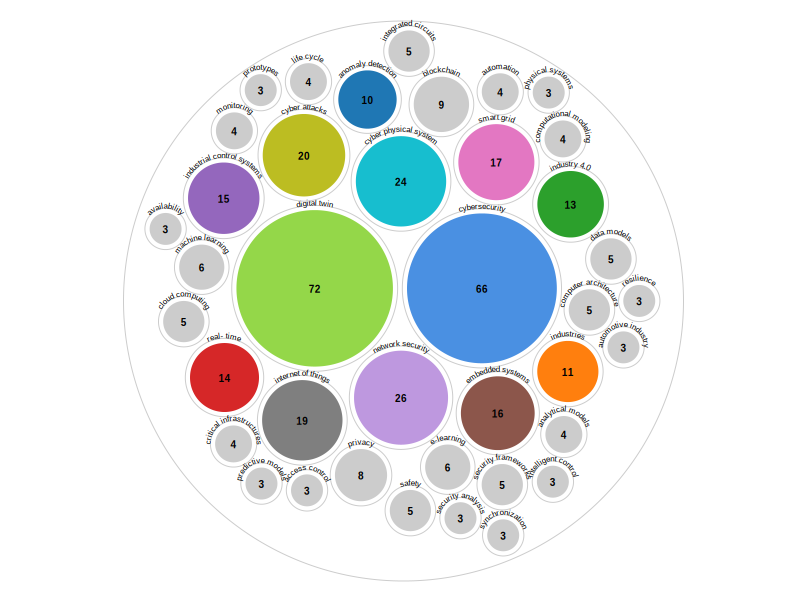
\includegraphics[width=\textwidth]{images/svg/key_buble.png}
    \includegraphics[width=1\linewidth]{images/rt/keywordoccurence.png}
    \caption{Frequency of Keywords from Keyword Section of 67 Papers}
    \label{fig:alluvial-key}
\end{figure}


'digital twin' with 55 occurrences indicates the centrality of this concept in this review. 'cybersecurity' is the second most frequently mentioned word, indicating the selected papers focus on using Digital Twin to provide security services. 'iot' is the third a frequent mention word with 19 times mention.   This highlights the significant role of this enabling technology in sending and receiving data to and from the Digital Twin environment. 

This analysis identified several key enabling technologies, namely 'blockchain(9),' 'machine learning(8)' 'cloud computing(4)' and 'analytics(3)'. These technologies are the main driving force of Digital Twin to be used as a security tool. 

Our frequency analysis also revealed the prevalent adoption of Digital Twin within Industry 4.0, as evidenced by terms such as 'cyber-physical systems(8)', 'smart grid(7)', and 'industrial control systems(6)'. These industry sectors highlight the integration and utilization of Digital Twin in critical infrastructure, indicating its role in providing various services including security-related functions. 


The main security and non-security functions of Digital Twin identified from the analysis were 'anomaly detection(7)', 'network security(6)', and 'simulation(6)'. This indicates the growing interest in leveraging Digital Twin frameworks for proactive security measures (anomaly detection), monitoring and detecting security problems in interconnected networks and utilizing simulation techniques for testing security measures before they are deployed to real operation environments to avoid accidental failure. 

\subsubsection*{Keyword Co-relationship Network}
In order to gain further insights into the evolution of research in the field of Digital Twin and cybersecurity, a keyword co-relationship network analysis was extracted from the VOSviewer tool. 

This analysis aimed to identify clusters of related items and visualise the relationships between keywords over time. The results of this analysis revealed that in the early days of research on Digital Twin, keywords such as "computational modelling", "embedded system", "situational awareness", "safety", and "simulation" were frequently mentioned, which suggests that the primary focus of the research at that time was on utilising Digital Twin as a visual aiding tool. 

On the other hand, more recent research was characterized by the frequent mention of emerging technologies such as "blockchain," "machine learning," "e-learning" "5G," and "emulation" This indicates that the development of Digital Twin has shifted towards utilising these technologies and augmenting Digital Twin to provide more service other than used as a model.



\begin{figure}[H]
    % \centering    
    \includegraphics[width=\textwidth, center]{images/newimages/vosviewer-2oc.png}
    % \includesvg[width=\textwidth]{images/new}
    % \includesvg[inkscapelatex=false,width=0.95\columnwidth]{images/key_belt.svg}
    \caption{keyword co-relationship from VOSviewer}
    \label{fig:co-occurrence-vosv}
\end{figure}

The analysis of the co-occurrence of keywords in the selected articles, as represented in Figure \ref{fig:co-occurrence-vosv}, identified eight clusters. As defined by the VOSviewer documentation, these clusters are groups of terms that exhibit a high degree of relatedness. 


\textit{Cluster One:}
This cluster focuses on various aspects related to the industrial and digital domains. It includes topics such as authentication, autonomous vehicles, cloud computing, costs, digital twin, industrial Internet of things (IIoT), microgrids, real-time systems resilience, and smart manufacturing. The common theme in this cluster appears to be the integration of digital technologies in industrial settings, emphasizing security, efficiency, and advanced manufacturing processes.

\textit{Cluster Two:}
This cluster revolves around computer-related topics, computational modelling, computer architecture, and embedded systems. It also includes subjects like cyber-physical systems, industry 4.0, network security, situational awareness, and smart grids. The primary focus here seems to be the intersection of computer science and engineering, with an emphasis on the integration of smart technologies into physical systems and networks.

\textit{Cluster Three:}
Cluster three is centered around security and privacy concerns in the digital landscape. It encompasses topics such as blockchain, cyber Digital Twin, cybersecurity, data privacy, safety, smart cities, smart contracts, soft sensors, and traffic control. The key theme here is the exploration of secure and privacy-preserving solutions in digital ecosystems, including blockchain technology and data protection measures.

\textit{Cluster Four:}
This cluster focuses on topics related to access control, automation, data security, and smart homes within the Internet of Things (IoT) context. The cluster includes items such as access control, automation, data security emulation, and IoT smart homes. The primary theme revolves around securing and managing access to IoT devices and systems, as well as exploring automation and smart home technologies.

\textit{Cluster Five:}
Cluster five centers on industrial control systems and security. It includes topics such as industrial control systems, integrated circuits, intelligent control, intrusion detection, machine learning, predictive models, and security-by-design. The focus here is on ensuring the security and reliability of industrial control systems, incorporating intelligent control algorithms, and leveraging machine learning for intrusion detection and predictive maintenance.

\textit{Cluster Six:}
This cluster encompasses topics related to communication networks and security frameworks. It includes items such as 5G, cyber range, industries, pipelines, security framework, security operation center, and wireless communication. The primary theme is the exploration of cyber range for training employees in sectors such as 5g network and security operation center. 



\textit{Cluster Seven:}
Cluster seven revolves around anomaly detection, cyber-physical systems, deep learning, monitoring, and SCADA systems. The focus here is on leveraging advanced techniques such as deep learning and anomaly detection for monitoring and securing cyber-physical systems, particularly in the context of SCADA systems.

\textit{Cluster Eight:}
Cluster eight is centered around analytical models, simulation, and testing. The focus is on the development and application of analytical models and simulation techniques for testing and evaluating various systems or scenarios.
%----------------------------------------------------------------------------------------

% \subsection{Study Selection and Refinement}
%----------------------------------------------------------------------------------------
% ======================================================================================================
% NOTES, TODOS
% ======================================================================================================
\subsection{Study Selection and Refinement}

After the screening of 452 papers using the inclusion/exclusion criteria, we were left with 83 papers. However, during the review phase, we excluded 16 more papers and we ended with 67 papers for further review and analysis. 


We had to exclude several papers during our review process for the following reasons:
\begin{itemize}
   \item \textbf{Irrelevant to (I)IoT and Industry 4.0}: Some papers were not relevant to securing applications related to \textbf{(I)IoT} with an \textbf{Industry 4.0} context. For instance, we came across a study that used a \textbf{Digital Twin} to secure a data center, which did not fit within our scope.

    \item \textbf{Duplicate Content}: We identified instances where the same study was submitted to different journals with different metadata, yet contained nearly identical content. Unfortunately, the tools we employed couldn't always catch these duplicates.
    
    \item \textbf{Non-Conference Source}: We excluded studies that were sourced from book chapters rather than conference proceedings, as they didn't align with our criteria.
    
    \item \textbf{Lack of Relevance to Research Questions}: Some studies simply weren't relevant to any of the research questions we were addressing.
    
    \item \textbf{Unrelated to Industry Use Case}: Studies that focused on securing \textbf{(I)IoT} devices without any connection to an industry use case were also among the excluded papers.
    
\end{itemize}

As a result of this refinement and selection process, the final set of 67 papers were identified for in-depth data extraction and analysis. In the subsequent section, we present a review of these papers, with a focus on addressing two research questions:\begin{itemize}
    \item[-] How is Digital Twin used to enhance security in Industry 4.0?
    \item[-] And what security mechanisms are used to secure the communication channel between Digital Twin and (I)IoT? 
\end{itemize} 

 





%----------------------------------------------------------------------------------------

% \subsection{Data Extraction and Monitoring}
%----------------------------------------------------------------------------------------
% ======================================================================================================
% NOTES, TODOS
% ======================================================================================================
\subsection{Data Extraction and Monitoring}
%----------------------------------------------------------------------------------------

% \subsection{Data Synthesis}
%----------------------------------------------------------------------------------------
% ======================================================================================================
% NOTES, TODOS
% ======================================================================================================
\section{Literature Review Result and Analysis}
In conducting this literature review, our primary objective is to answer two research questions related to the use of Digital Twin to enhance security in Industry 4.0. The first research question aimed to identify existing solutions that leverage Digital Twin to improve security in the use cases of Industry 4.0, while the second question aimed to identify the mechanisms used to secure communication between Digital Twin and (I)IoT devices.

In this paper, we followed the three-phase approach outlined by Kitchenham and Charter \cite{kitchenham_guidelines_2007} to perform a systematic review of the literature. We leveraged automating tools, including Parsif.al for designing our review protocol, VOSviewer for conducting bibliometric analyses, and Logseq for data collection and to facilitate the review process.

We began by searching six different digital libraries and collecting a total of 727 papers. We then applied inclusion and exclusion criteria, as well as a study refinement phase, to arrive at a final selection of 67 items that are relevant to answer the first two research question.

To ensure consistency in our review process, we developed a data extraction form as described in table \ref{tbl:extraction}. This approach allowed us to systematically analyze each of the selected papers and provide insights into the application of Digital Twin technology in Industry 4.0 use cases.

% ======================================================================================================
% NOTES, TODOS
%
% ======================================================================================================
%
\subsection{RQ1: { Digital Twin as Security Tool in Industry 4.0}}
\label{sec:rq1dtsec}
This subsection aims to answer the first research question of this paper which is how digital twin is used to provide various security services in Industry 4.0. 

Though the integration of operational technology and IT systems in Industry 4.0 increases the risk of cyber attacks \cite{rajivfaleiroDigitalTwinCybersecurity2022}, technologies like Digital Twin offer possibilities to improve security \cite{dietzHarnessingDigitalTwin2022}. In fact, the literature review also suggests that Digital Twin can be applied to enhance security in Industry 4.0 applications across multiple sectors. Table \ref{tbl:lit-bench} summarizes some of the research contributions that show the use of Digital Twin to improve the security of Industry 4.0 in various domains. 

The research papers were classified and analysed based on several criteria, including the target sector (use case), the purpose of DT, the enabling technology used (integrated with DT), the contribution (category of methodology), and the type of study (characteristics of the study). The table demonstrates the wide range of sectors in which Digital Twins can be applied to improve security in industries including satellite, energy, power grid, intelligent transport systems, water, agriculture, the automotive industry, and manufacturing.

The Enabling technologies used in the studies include big data,  AI(machine learning), cloud computing and data analytics, edge computing, blockchain, and NFV, among others. These technologies enable researchers to build DT-based systems equipped with security features for various use cases.

The contributions of the studies were identified as frameworks, platforms, and architectures. We classify a contribution as a platform if the research presents a tool that can be deployed and used to provide security services like intrusion detection. If the authors provide only a high-level overview of the proposed solution, we classify it as an architecture. On the other hand, if details are presented for each component of the architecture, we classify it as a framework.

Regarding the study types, Table \ref{tbl:lit-bench} shows that there are theoretical studies, case-based and experimental-based studies, and review-type studies. Theoretical studies tend to focus on proposing conceptual frameworks and architectures. And case-based studies tries to provide solutions targeting specific industry sectors. Whereas experimental studies tend to evaluate the proposed frameworks and algorithms through an experiment and proof of concept. Note that a study can be both case-based and experimental if an experiment is performed on a target industry sector. 

% \begin{adjustwidth}{-0.5in}{}
% \begin{minipage}{\textwidth}

% \begin{table}[H]
% \tiny
% \centering
% \caption{\label{tbl:lit-bench} Overview of References by Use Case, Purpose of Digital Twin, Enabling Technology, Contribution Category, and Study Type.}
% % \resizebox{\linewidth}{!}{
% \renewcommand{\arraystretch}{2.0} % Increase the row height by a factor of 1.5
% \begin{NiceTabular}{p{0.1cm}p{2.5cm}p{2.5cm}p{2cm}p{3cm}p{1.5cm}}
% \CodeBefore
% % \rowcolors[gray]{2}{0.8}{}[cols=1-2,restart]
% \Body
% \toprule
%     \textbf{Ref}  & \textbf{Use Case}& \textbf{Purpose} & \textbf{Enabling Technology }  & \textbf{Contribution Category} & \textbf{Study type} \\
%     \midrule

   
    
% \bottomrule
% \end{NiceTabular}
% % }
% \end{table}

% --------------------------------------------
\begin{longtblr}[
  caption = {Digital Twin: Use Cases, Purpose, Enabling Technology, Contribution Category, and Study Type in References},
  label = {tbl:lit-bench},
]{
  colspec = {|X[0.5cm]|X[2cm]|X[2.9cm]|X[3cm]|X[2cm]|X[2cm]|},
  rowhead = 1,
  hlines,
  row{even} = {gray9},
  row{1} = {olive9},
  row{1-Z} = {1em,font=\small}
} 
\textbf{Ref}  & \textbf{Use Case}& \textbf{Purpose} & \textbf{Enabling Technology }  & \textbf{Contribution Category} & \textbf{Study type} \\

    \cite{salimBlockchainEnabledSecureDigital2022} & Smart manufacturing & Botnet detection & ML and Blockchain & Framework & Experiment \\

    \cite{xiaoCommandFenceNovelDigitalTwinBased2022} & Smart Home & Intrusion detection and prevention & Deep Learning ( Deep Q-Network) & Platform & Experiment \\
    
    \cite{pirbhulalNovelFrameworkReinforcing2022} & Healthcare & Vulnerability Assessment/Testing & - & Framework & Theoretical \\
    
    \cite{marksteinerUsingCyberDigital2021} & Automotive & Black-box Testing & - & Framework & Theoretical \\
    
    \cite{dietzIntegratingDigitalTwin2020} & ICS & Attack Testing & Analytics & Framework & Experiment \\
    
    \cite{grasselliIndustrialNetworkDigital2022} & CPS & Risk Assessment/Testing & cloud Computing, Network Function Virtualization(NFV) & Architecture & Theoretical \\
    
    \cite{guoCyberSecurityRisk2021a} & Nuclear Plant & Testing & 3D Modeling, Software Defined Network (SDN) & - & Theoretical \\

    
    \cite{jiaqiliSpaceSpiderHyper2022} & Satellite & Simulation & Big Data and AI & Platform & - \\
     
     \cite{danilczykSmartGridAnomaly2021} & Smart grid & Anomaly detection & Machine Learning & Architecture & Experiment \\

    \cite{shitoleRealTimeDigitalTwin2021} & Energy & Testing & - &  Platform & Case-Study \\

    \cite{saadImplementationIoTBasedDigital2020} & Power grid & Anomaly detection & Cloud Computing and Data Analytics & Framework and Algorithms & Experiment based \\
    
    \cite{akbarianIntrusionDetectionDigital2020} & ICS & Simulating and Testing & Machine Learning & Algorithm & Experiment \\

    \cite{dietzHarnessingDigitalTwin2022} & ICS & Simulation & - & Framework and Algorithms & Experiment \\

    \cite{eckhartEnhancingCyberSituational2019} & CPS & Monitoring, Incident Handling, Testing & - & Framework & Theoretical \\

    \cite{maillet-contozEndtoendSecurityValidation2020} & Water, Agriculture & Simulation and Testing & Data Analytics & Architecture & Case study and Experiment \\

    \cite{giovannipaolosellittoEnablingZeroTrust2021} & Smart Grid & device policy enforcement & - & Architecture & Theoretical \\

    \cite{dietzEmployingDigitalTwins2022} & ICS & Testing and Security Assessment & - & Framework & Experiment \\

    \cite{sousaELEGANTSecurityCritical2021} & ICS & Intrusion Detection & Machine Learning & Architecture & Experiment \\

    \cite{xuEfficientAuthenticationVehicular2021} & Automotive Industry & - & - & Framework and Algorithm & Theoretical \\
    
   \cite{bittonDerivingCostEffectiveDigital2018a} & ICS & Testing & - & Framework & Experiment \\
   
   \cite{glenandbensonjamesandguptamaanakandsandhuravicatheyEdgeCentricSecure2021} & Intelligent Transportation & Access Control & Edge Computing & Architecture & Case-study \\

   \cite{wangDTCPNDigitalTwin2022} & Enterprise Network & Simulation & NFV, Big data processing & Platform & Experiment \\

   \cite{franciaDigitalTwinsIndustrial2021} & ICS & Testing, Vulnerability assessment & - & - & Experiment \\

   \cite{lopezDIGITALTWINSINTELLIGENT2021} & Smart Grid & Detection & Blockchain & Architecture & Theoretical \\
    
   \cite{adrienbacueDigitalTwinsEnhanced2022} & Aerospace & Simulation(Attack) & - & - & Case-study \\
    
   \cite{veledarDigitalTwinsDependability2019} & Automotive industry & Predictive analytics & - & Platform & - \\

   \cite{holmesDigitalTwinsCyber2021} & - & - & - & - & Review paper \\

   \cite{vargheseDigitalTwinbasedIntrusion2022} & ICS & Intrusion Detection & Machine Learning & Framework & Experiment \\

   \cite{rajivfaleiroDigitalTwinCybersecurity2022} & - & - & - & - & Review paper \\

   \cite{hossenDigitalTwinSelfSecurity2021} & Power Grid & Model & - & Algorithm & Experiment \\

   \cite{luongnguyenDigitalTwinIoT2022} & Intelligent Transport System & Testing and Simulating & - & Platform & Case-study and Experiment \\

    \cite{almeaibedDigitalTwinAnalysis2021} & Automotive Industry & - & Analytics & Framework & Case-study \\
    
    \cite{becueCyberFactorySecuringIndustry40with2018} & Manufacturing & Simulation Testing-Training & - & Theoretical \\ 

    \cite{wuDeepLearningDriven2022} & CPS of Drones & Simulation & AI - Deep Learning & Model & Experiment \\

    \cite{salviCyberresilienceCriticalCyber2022} & Power Grid & Situational Awareness & Data Analytics & Model & Theoretical \\

    \cite{chukkapalliCyberPhysicalSystemSecurity2021} & Agriculture sector & Anomaly detection & Machine Learning & Framework & Experiment \\

    \cite{hadarCyberDigitalTwin2020} & Enterprises & - & Analytics & - & Experiment \\

    \cite{kumarBlockchainDeepLearning2022} & IIoT Network & Simulation, Intrusion Detection & Blockchain, Deep Learning & Framework & Experiment \\

    % \cite{sugumarAssessmentMethodDetecting2019} & Water Treatment Plant & Assessment , Simulation & - & Model & - \\
    % \hline

    \cite{williamdanilczykANGELIntelligentDigital2019} & Smart Grid & Data Visualization & - & Framework & Experiment \\

    \cite{masiSecuringCriticalInfrastructures2023} & Intelligent Transport Systems & - & - & Architecture & - \\

    \cite{kandasamyElectricPowerDigital2022} & Smart Grid & Training & - & Platform & Case-study \\

    % \cite{hussainiTaxonomySecurityDefense2022} & Smart Industries & Simulation and Intrusion Detection & Architecture & Case-study \\
    % \hline

    \cite{akbarianSecurityFrameworkDigital2021} & ICS & Intrusion Detection & Cloud Computing & Framework, Algorithm & Experiment \\

    % \cite{xuGametheoreticApproachSecure2020} & CPS & Fault detection, Monitoring & - & Framework & Experiment \\
    % \hline

    \cite{atalayDigitalTwinsApproach2020} & Smart Grid & Testing & - & Framework & Theoretical \\

    \cite{houDigitalTwinRuntime2022} & Satellites and Space & Penetration Testing & - & Framework and Algorithm & Theoretical \\

    % \cite{vakarukDigitalTwinNetwork2021} & Telecom & Training & Machine Learning & Platform & Theoretical \\
    % \hline

    \cite{rebecchiDigitalTwin5G2022} & 5G Network & Simulation - Training and Testing & Machine learning & Architecture & Experiment \\

    \cite{gehrmannDigitalTwinBased2020} & ICS &  Data sharing & - & Model, Architecture & Case study \\

    \cite{chengzhelaiSPDTSecurePrivacyPreserving2022} & Transportation & - & Cloud & - & - \\
    
    \cite{vielberth2021digital} & CPS & Training & - & Platform & Experiment \\
    
    % \cite{olivares-rojasCybersecuritySmartGrid2022} & Power grid & Testing & - & Framework & Theoretical \\
    % \hline

    \cite{suhailSituationalAwareCyberphysical2022} & Automotive industry & Testing & Blockchain & Framework & Use-case \\
    
    \cite{harrisonCybersecurityThreatModeling2022a} &  Automotive & Threat Modeling, Testing & Analytics & - & Experiment \\

    \cite{aryaDetectionMaliciousNode2023a} &  Transportation & Detection & Machine learning & Framework & - \\
    
    \cite{wangDigitalTwinNetwork2022a} &  5G Network & Detection & - & Framework & - \\

    \cite{xuDigitalTwinbasedAnomaly2023a} &  CPS & Anomaly Detection & Machine Learning & Framework & Case Study \\
    
    \cite{dietzUnleashingDigitalTwin2020} &  ICS & Simulation, Testing & - & - & - \\
    
    % ... more rows ...
    \cite{epiphaniouDigitalTwinsCyber2023a} & CPS/IoT & Security Assessment & AI and Modeling and Simulation Tools & - & Experiment through Proof of Concept \\
    
    \cite{ayyalusamyHybridDigitalTwin2022a} & Smart Power Grid & Vulnerability Assessment & MATLAB-SIMULINK, Node-RED & Architecture & Experiment through test-bed\\
    
    \cite{sunResearchSecurityManagement2021a} & Power Grid & Security Management & Edge Computing & Architecture & Theoretical\\
    
    \cite{vanderwalSecuringNetworksIoT2022a} & IoT & Vulnerability Assessment & Automated Adversary Emulation \textit{(Caldera)} & Architecture & Experiment\\

    % ----------------------------------------
    \cite{liuDistributedCollaborativeAnomaly2021} & Vehicular Network/ Automotive & Anomaly Detection & Machine Learning, Edge Computing & Architecture & Experiment\\
    

\end{longtblr}

Note that, the data extracted using extraction form from Table \ref{tbl:extraction} and presented in Table \ref{tbl:lit-bench} doesn't include data from papers that focus only on securing the data used by Digital Twin technology.  


%----------------------------------------------

% \begin{center}
% \begin{figure}
% \begin{adjustwidth}{-5cm}{3cm} % Set the left margin to 2cm
% \hspace*{-4.5cm}
% \begin{longtable}{p{0.5cm}p{2cm}p{2.9cm}p{3.0cm}p{3.0cm}p{2.0cm}}
%     \caption{\label{tbl:lit-bench} Overview of References by Use Case, Purpose of Digital Twin, Enabling Technology, Contribution Category, and Study Type.} \\
%     \toprule
%     \textbf{Ref}  & \textbf{Use Case}& \textbf{Purpose} & \textbf{Enabling Technology }  & \textbf{Contribution Category} & \textbf{Study type} \\
%     \hline
%     \endfirsthead
%     \endhead
    
% \end{longtable}
% \end{adjustwidth}
% \end{figure}
% \end{center}
% % ======================================================================================================
% NOTES, TODOS
% Explain how digital twins evolve 
% Why it was incepted in the first place
% What is the potential gain of digital twins...monitoring, optimization..etc
% Prepare a table that shows the definition of DT and the corresponding paper.
% ======================================================================================================
%
\subsection{Exploring the Concept of Digital Twin}

The concept and definition of digital twins have been subject to various interpretations by researchers and scholars, contingent upon the specific context. Nevertheless, the essential components of a digital twin can be generally characterized by 3 main components: two states(physical and digital), inter-connectivity (the channel between the two states), and process( a mechanism for collecting and examining data). In this section, we endeavor to provide a comprehensive definition of digital twins by synthesizing a definition derived from a  review of 30 research papers on the topic. The definition and respective reference are listed in Table \ref{tbl:dtconcept}

Here we give a complete definition of digital twins from a collection of various definitions of research publications: \textit{ Digital Twin is a virtual representation of a physical object or system that mirrors its real-world counterpart through real-time updates and tracking of its entire life-cycle. It is designed to model the physical characteristics and behaviors of the object using digital technology, mapping the physical operating environment to virtual space for interaction and providing valuable insights through collecting asset-centric data, analytic capabilities, and simulations. Digital twins are used for monitoring, simulating, optimizing, and predicting the state of the physical object. They have a standard structure, end-to-end connectivity, communication protocol with backward compatibility, and standard data format for communication between the twins.}

\begin{table}[H]
\scriptsize
\centering
\caption{\label{tbl:dtconcept} Definition of digital twin in the literature}
\begin{NiceTabular}{p{10cm}|p{4cm}}
\CodeBefore
% \rowcolors[gray]{2}{0.8}{}[cols=1-2,restart]
\Body
\toprule
    \textbf{DT definition} & \textbf{Reference(s)} \\
    \midrule
     Digital twins are virtual representations of industrial assets that provide valuable insights through collecting asset-centric data, analytic capabilities and simulations & \cite{dietzIntegratingDigitalTwin2020, eckhartEnhancingCyberSituational2019} \\  
     \hline
    A virtual representation of a physical system, process, or product that is synchronized with its real-world counterpart & \cite{gehrmann_digital_2020, rebecchiDigitalTwin5G2022} \\ 
    \hline
    It is used as a virtual representation of a physical entity, modelling its components and properties & \cite{vakarukDigitalTwinNetwork2021} \\
    \hline
    A system that continuously monitors the physical state of an environment through wide sensor arrays and compares it to simulation models to gain deeper insights into its operating condition & \cite{williamdanilczykANGELIntelligentDigital2019, xuGametheoreticApproachSecure2020, danilczykSmartGridAnomaly2021, veledarDigitalTwinsDependability2019, kumarBlockchainDeepLearning2022, hadarCyberDigitalTwin2020} \\
    \hline
    A virtual representation of a physical system, process or product that is synchronized with its real-world counterpart & \cite{gehrmann_digital_2020, luongnguyenDigitalTwinIoT2022, lopezDIGITALTWINSINTELLIGENT2021} \\ 
    \hline
    A technology to map the physical operating environment to virtual space for interaction. & \cite{wuDeepLearningDriven2022}  \\ 
    \hline
    Evolving digital profile of the historical and current value of physical object or process. & \cite{becueCyberFactorySecuringIndustry40with2018} \\
    \hline

    Virtual representation of physical objects or systems that can be used to monitor and control the real-world counterparts & \cite{almeaibedDigitalTwinAnalysis2021, chukkapalliCyberPhysicalSystemSecurity2021, dietzEmployingDigitalTwins2022}\\
    \hline
    virtual replica of physical object with standard structure, end-to-end connectivity, communication protocol with backward compatibility, and standard data format for communication between the twins & \cite{atalayDigitalTwinsApproach2020} \\

    \hline
    DT is a mapping between physical object and virtual entity that receive data in real-time to predicate the state of the physical object & \cite{dinglingsuzehuiquDetectionDDoSAttacks2022} \\
    
    \hline
    A virtual Model designed to accurately map a physical object or process & \cite{wangDTCPNDigitalTwin2022, sousaELEGANTSecurityCritical2021} \\
    
    \hline
    a method to describe and model the physical characteristics and behaviors of physical objects by using digital technology & \cite{wangSoCbasedDigitalTwin2020} \\
    
    \hline
    A virtual space for representation of real world object and an information flow to keep them synchronize  & \cite{giovannipaolosellittoEnablingZeroTrust2021}\\
    
    \hline
    A digital twin is a virtual representation of a physical object that tracks and mimics its entire life-cycle through real-time updates & \cite{vargheseDigitalTwinbasedIntrusion2022, dietzUnleashingDigitalTwin2020} \\
    
    \hline
    Digital Twin is a virtual replica of physical system that precisely mirror the internal behavior of system for monitoring, simulating, optimizing and predicating the state of the system & \cite{akbarianSecurityFrameworkDigital2021, akbarianIntrusionDetectionDigital2020} \\
    
    \hline
    a digital twin is defined as an integrated system that combines computational, communication and physical aspects of Cyber Critical Infrastructures (CCIs) to provide increased cyber situational awareness & \cite{salviCyberresilienceCriticalCyber2022, pirbhulalNovelFrameworkReinforcing2022} \\

    \hline
    
    
\bottomrule
\end{NiceTabular}
\end{table}


% ======================================================================================================
% NOTES, TODOS
% Telecommunication -> 1, 2
%     5G network 
% Power grid, smart grid Energy sector-> 3, 4, 5
% Transportation -> 1, 2
% Agriculture sector
% Automotive -> 1, 2
% Water treatment -> 1
% Space industry -> 1
% General
%     Industry Control system -> 1, 2
%     Cyber-Physical System -> 1, 2, 3, 
%     IIoT network -> 1
%     Digital Enterprises  -> 1
%     smart manufacturing -> 1

% ======================================================================================================


% In this systematic literature review, we categorised the papers based on the industry sector they targeted. To avoid bias classification, we followed a systematic way of identifying the target industry based on the following condition. 

% \begin{itemize}
%     \item If the authors explicitly specify the industry for which their proposed solution is targeted, we consider this to be the target industry of the paper.
%     \item In cases where the target industry was not explicitly mentioned, we looked at the experiments and use cases presented in the paper to identify the targeted industry.
%     \item If we couldn't find the target industry through the previous methods, we searched for any discussions of Industrial Control Systems (ICS) or Cyber-Physical Systems (CPS) in the paper, and if found, we categorised the paper under ICS/CPS.
% \end{itemize}

% Note that, from the initial pool of 67 papers,  our categorization approach excluded studies that solely focused on providing security mechanisms for digital communication between Digital Twin and (I)IoT. 


% Upon the completion of our categorization process, we have identified the following primary industry sectors illustrated in Figure \ref{fig:use-dt}. \\
% % Power grid, Agriculture, health, Smart home, Transportation, Autonomous Vehicle, Water Treatment, Space industry, Smart Factory, Automotive industry, 

% \begin{center}
 

% \smartdiagram[constellation diagram]{
%   DT,
%   Power grid, Agriculture, Health, Smart home, Transportation, Automobile/vehicle, Water Treatment, Space industry, Smart Factory, Automotive industry
% }
% \captionof{figure}{Use Cases Of DT}
% \label{fig:use-dt}
% \end{center}

% Our finding revealed that Digital Twin-based security solution has been widely adopted in several industries ranging from Smart Grid(SG) to Smart Homes(SH) for various purposes. Intrusion detection \cite{akbarianIntrusionDetectionDigital2020}, anomaly detection, training and testing \cite{rebecchiDigitalTwin5G2022,becueCyberFactorySecuringIndustry40with2018}, botnet detection \cite{salimBlockchainEnabledSecureDigital2022}, etc. are among the main functions provided through this digital technology. 

% In the following section, the usage of Digital Twin as a security tool in the major industry 4.0 sector is presented. 

\subsubsection*{Power Grid}
The study by Danilczyk et al.\cite{williamdanilczykANGELIntelligentDigital2019} proposed a framework named "Automatic Network Guardian for Electrical Systems (ANGEL) which uses real-time data visualization to enhance the security and resiliency of microgrids. The framework models both the cyber and physical layers of the microgrid, allowing it to detect discrepancies between simulated and physical systems under various operating conditions. The framework's two-way coupling between the simulation and the physical system enables it to update and improve its simulations, detect unnatural changes, and evaluate meter data accuracy, thereby improving security. ANGEL can also be equipped with machine learning to have self-healing capabilities that can mitigate component failures and cyber-attacks. While the ANGEL framework is promising, it has limitations, including potential false positives and difficulty detecting some types of malicious attacks. Additionally, the framework is still in development and has not yet been tested on a real-world microgrid system for further evaluation.

Another study by Saad et al.\cite{saadImplementationIoTBasedDigital2020} presents an IoT-based Digital Twin for microgrids that aim to improve their resilience against cyber attacks. The proposed framework is implemented as a cloud-based Digital Twin platform that acts as a central hub for the networked microgrid system. It is designed to model both the physical and cyber layers of the microgrid, allowing it to detect false data injection (FDIA) and denial of service (DoS) attacks. The framework utilizes observer-based What-If scenarios to take corrective action when an attack is detected, ensuring the safe and seamless operation of the networked microgrids. The proposed Digital Twin framework is validated using a practical setup of the distributed control system and Amazon Web Services (AWS) and is able to quickly detect and mitigate a range of cyber attacks. The authors argue that combining deep learning and Luenberger Observer(LO) enhances the speed, accuracy, and predictability of attacks. In general, the proposed IoT-based Digital Twin framework presents a practical solution to improve the resilience of microgrids against cyber attacks.

 % that evaluates the incoming power setpoints for safety before implementation. The algorithm utilizes the steady-state and dynamic behaviours of the inverter. The dynamic behaviour was experimentally determined using a laboratory setup. The study demonstrated the Digital Twin formed using an algorithm that encompasses the inverter's steady-state and dynamic response models, can help to protect smart grids from man-in-the-middle attacks. This was achieved by  incoming commands via the Digital Twin before engaging them in the local controller.

In\cite{hossenDigitalTwinSelfSecurity2021} paper, Hossen et al. propose a knowledge-based self-security algorithm that leverages the inverter's steady-state and dynamic behaviours, determined experimentally, to create a Digital Twin. This Digital Twin acts as a virtual replica of the inverter and is employed to evaluate incoming power setpoints for safety prior to their implementation. The approach's main objective was to safeguard smart grids from man-in-the-middle attacks. By thoroughly examining incoming commands via the Digital Twin before involving the local controller, the method effectively prevents unsafe setpoints from being implemented.

The study undertaken by Atalay et al.\cite{atalayDigitalTwinsApproach2020} focuses on providing an overview of smart grid cybersecurity standards and reviews major threats to smart grid environments at the physical, network, and application layers. In this study, the authors argue that despite the prevalence of smart grids in energy distribution networks, there is a lack of standards for comprehensive security assessment, which is a critical shortcoming. With the aim to address this gap, the authors propose a Digital Twins-based approach for the security testing lifecycle of smart grids, by accurately modelling the functioning of the physical grid and running security testing on the model without causing disruption. This approach has the potential to become an important tool for standardisation. While the paper presents an innovative framework for security testing, it lacks experimental validation and implementation details for real-event scenarios.


In their study, Sellitto et al.\cite{giovannipaolosellittoEnablingZeroTrust2021} proposed a methodology to build a cybersecurity Digital Twin of a Smart Grid based on its architectural blueprint. The methodology aims to enable the adoption of Zero Trust Architecture (ZTA) and dynamic enforcement of security policies for devices connected to the grid. The authors presented a novel approach to dynamically align the Digital Twin with its real-world counterpart, creating a maintenance-aware model for the Smart Grid. This was achieved by adopting an architectural view that gets dynamically aligned with the state of the real-world counterpart during deployment and operation time. The authors laid the foundation for a Digital Twin model that allows dynamic enforcement of security policies that reflect Smart Grid topology changes over time. 


Salvi et al.\cite{salviCyberresilienceCriticalCyber2022} targets the electrical energy sector with the aim of increasing the cyber-resilience of Critical Control Infrastructures (CCIs) using a Digital Twin implementation to address risks associated with the integration of computational, communication, and physical aspects of CCIs. It seeks to provide increased situational awareness, a common understanding of incidents, and enhanced response capacity to minimize response time and reduce the impact of cyber-attacks on organizations and society. However, the study is limited by the fact that it only focuses on the conceptual model, rather than the implementation of the DT, which may require further validation through proof of concepts in different CCI contexts. Nevertheless, this research addresses the needs expressed by key stakeholders in the electrical energy sector and presents design principles that can be applied in disaster management contexts.


A study by Danilczyk et al.\cite{danilczykSmartGridAnomaly2021} presents a deep-learning convolutional neural network (CNN) as a module within the Automatic Network Guardian for Electrical Systems (ANGEL) Digital Twin environment to detect physical faults in a power system. The approach uses high-fidelity measurement data from the IEEE 9-bus and IEEE 39-bus benchmark power systems to detect if there is a fault in the power system and to classify which bus contains the fault. The anomaly detection CNN algorithm was able to identify the existence of a fault with near-perfect accuracy and classify the location of the fault with an accuracy of nearly 95\% for both systems. The long-term goal of this project is to have the Digital Twin with the anomaly detection CNN running alongside the physical smart grid. However, the study's limitation is that, due to the small timescales present in power systems, the inference speed of the network will be of critical importance. For real-time implementation, more powerful hardware would be beneficial to the overall performance of the integrated system. Despite this limitation, deep learning algorithms show significant promise in the detection and location of power system faults and can improve performance and reduce the cost of power distribution.

To overcome limitations in security studies of Smart Grids (SG) in physical test beds Kandasmy et al.\cite{kandasamyElectricPowerDigital2022} build a digital power twin that enables the deployment of real-world attacks and countermeasures while allowing easy modification of components and configurations. The tool presented by the authors, named EPICTWIN, a Digital Twin for a power physical test-bed, allows users to validate the security and safe operation of critical components in a more realistic environment, reducing the gap between physical and simulated test-bed environments. They claim their tool provides an attacker designer(AD) and attack launcher(AL), unique tools that enable researchers to validate and improve defence mechanisms even without expertise in offensive security testing. Finally, the authors highlight the uniqueness of their contributions in building a Digital Twin of an existing cyber-security test bed, presenting a procedure that can be extended to any type of system, and providing unique tools for launching systematic attacks on the twin.

In \cite{sunResearchSecurityManagement2021a} this study, the authors' contribution lies in proposing a security management and control model for the power grid digital twin using edge computing technology. They highlight the increasing demand for power grid security and the vulnerabilities posed by edge computing and digital twin technologies and construct a power grid digital twin security control model, consisting of five layers: application layer, function layer, model layer, data layer, and physical layer. This model aims to ensure all aspects of the power grid are protected, allowing for efficient and safe operation in a technology-driven environment. The authors emphasize the importance of data layer security due to the risk of data loss and tampering in the power grid context. They also discuss the mutual coupling between physical entities and virtualized objects in the power grid digital twin's physical layer, supporting practical applications like equipment detection, fault alarm, and maintenance planning.


The authors of this \cite{ayyalusamyHybridDigitalTwin2022a} research paper proposes a Hybrid Digital Twin (HDT) system for cyber security analysis in smart grids and other cyber-physical systems. The HDT system comprises a MATLAB-SIMULINK digital model representing the physical system and multiple single-board computers representing the cyber components. The Digital Twin is used in this research to identify the cyber-security vulnerabilities in smart grids and other cyber-physical systems. The HDT can replicate real industrial hardware and network components by establishing highly configurable, low-cost, and scalable prototypes. The paper describes the HDT architecture and communication system design, including network segmentation using a configurable network switch and communication protocols using Node-RED. Performance evaluations show acceptable results for communication between digital and physical models and among network components. The HDT offers a platform for conducting cyber-security analyses in complex cyber-physical systems, addressing the challenges in securing power grids and other critical infrastructure.







\subsubsection*{Smart Factory}
Lopez et al.\cite{lopezDIGITALTWINSINTELLIGENT2021} aim in their research to analyze the evolution of digital twins in smart grid infrastructures and their role in implementing intelligent authorization policies. The authors study the application of AI technologies, including machine learning and blockchain, in the context of digital twins to manage dynamic information flows and detect cybersecurity issues in real-time. They provide a mid-term and long-term analysis of the pending challenges of DTs and discuss the three-stage process of Digital Twin evolution, starting from monitoring systems with limited analysis capabilities to fully semantic, self-learning platforms. The contribution of this article lies in the analysis of the future smart grid through the evolution of digital twins, pointing out the most relevant challenges they face. The authors conclude that digital twins will play a fundamental role in driving the progress of the electricity grid toward a fully decentralized and autonomous model, governed by intelligent authorization systems. However, standardization and information security efforts are necessary, along with deep research into machine learning specifically applied to critical infrastructures and smart cities.


 In\cite{shitoleRealTimeDigitalTwin2021} paper presented by Shitole et al. aims to develop a low-cost Real-Time Digital Twin (RTDT) of an interconnected and distributed Residential Energy Storage System (RESS) controlled and monitored via Cloud-based Energy Management System (CEMS), in order to analyse the cyber-security of such systems and develop appropriate Intrusion Detection Systems against cyber attacks. The proposed RTDT allows for flexibility in modifying, scaling, and replicating the system without compromising its real-time fidelity. The development procedure can be easily replicated to develop RTDT of any Cyber-Physical System (CPS) or micro-grid test-beds. The paper presents a systematic procedure for the development of the RTDT and verifies its performance through an experimental case study. The RTDT is developed using a low-cost single-board computer with Simulink Desktop Real-Time, which reduces overall development costs. Overall, this paper presents a reliable and economical solution for cyber security studies on RESS through the development of an RTDT.


 Salim et al.\cite{salimBlockchainEnabledSecureDigital2022} propose a secure blockchain-enabled digital framework for the early detection of botnet formation in a smart factory environment. The proposed framework integrates a Digital Twin (DT), a packet auditor (PA), deep learning models, blockchain, and smart contracts(SC) for securing the data flow of a smart factory environment. The Digital Twin is designed to collect device data and inspect packet headers for connections with external unique IP addresses with open connections. Data is synchronised between the Digital Twin and the PA for detecting corrupt device data transmission. Smart contracts-based Digital Twin and PA authentication is used to ensure malicious nodes do not participate in data synchronisation. Botnet spread is prevented using Digital Twin certificate revocation. A comparative analysis with existing research shows that the proposed framework provides data security, integrity, privacy, device availability, and non-repudiation.


In \cite{becueCyberFactorySecuringIndustry40with2018} paper by Bécue et al. discuss ITEA initiative CyberFactory\#1 project, which aims to develop a system of systems to optimize and ensure the resilience of digital factories and factories of the future (FoF) in the face of increasing digitization and connectivity. The project focuses on optimising the efficiency and security of the network of factories, proposing novel architectures and methodologies to address cyber and physical threats and safety concerns. It also integrates technical, economic, human, and societal dimensions. This study uses Digital Twin to support cybersecurity testing and training, together with cyber ranges, to enable risk anticipation and accurate impact prediction. The project demonstrates key capabilities in realistic environments and reflects the variety of possible new factory types and business model shifts.



\subsubsection*{Health}
An automated framework for improving cybersecurity in IoT-based healthcare applications using Digital Twin that includes innovative healthcare security techniques such as system modelling, traffic and attack generation, impact assessment, attack and response strategies, and cyber-attack prevention processes proposed by Pirbhulal et al.\cite{pirbhulalNovelFrameworkReinforcing2022} The authors investigate the applicability of Digital Twin for cyber-attacks prevention and present a strategic procedure for enhancing cybersecurity. The proposed framework can help update access control policies and enhance cybersecurity, and it provides an automated cybersecurity solution by incorporating system models and resolving known vulnerabilities and threats. However, the limitation of this research is that it is a theoretical study and needs to be validated through experiments and simulations. The authors conclude that Digital Twin is a valuable tool for enhancing cybersecurity in healthcare systems, as it provides analysis, design, and optimisation of systems to improve accuracy, speed, and effectiveness, and it can simulate security breaches and develop decision-making and mitigative responses to simulated cyberattacks. 

\subsubsection*{Smart Home}
% The design and implementation of a Digital Twin system for smart metering systems (SMS) in a smart home setting are presented in the work by Olivares-Rajos et al.\cite{olivares-rojasCybersecuritySmartGrid2022}. The system is mainly composed of a Digital Twin framework controller (DTFC) responsible for mapping real objects with its virtual representation, exchange values between DTs, notify events and alarms between all the objects, and simulating cyber threats and attacks. The SMS is mainly composed of an Smart Meter(SM) in the premises of the end-users, data concentrator (DC) that collect the SM consumption/production data, and metering database management system (MDMS) server that store all the information collected by DC. The authors conclude that the use of digital twins (DTs) is feasible in various contexts of the smart grid, particularly in cybersecurity testing.

In their\cite{xiaoCommandFenceNovelDigitalTwinBased2022} paper,  Xiao et al. propose a novel digital-twin-based security framework, CommandFence, to protect smart home systems from malicious and benign apps with design flaws or logical errors that may cause harm to the user when executed. The framework uses an Interposition Layer to interpose app commands and an Emulation Layer to execute these commands in a virtual smart home environment and predict whether they can cause any risky smart home state when correlating with human activities and environmental changes. If a sequence of app commands can potentially lead to a risky consequence, they are treated as dangerous, and the framework drops them before any insecure situation can occur. The authors fully implemented the CommandFence framework and tested it on 553 official SmartApps on the Samsung SmartThings platform, 10 malicious SmartApps created by Jia et al., and 17 benign SmartApps with logic errors developed by Celik et al. The experiment successfully identified 34 potentially dangerous SmartApps out of 553 official SmartApps, 7 out of 10 malicious SmartApps, and achieved 100\% accuracy for the 17 benign SmartApps with logic errors.CommandFence is orthogonal to the well-received permission-based access control mechanisms and can be implemented as plug-in software without any hardware upgrades. 

\subsubsection*{Transportation}

Cathey et al.\cite{glenandbensonjamesandguptamaanakandsandhuravicatheyEdgeCentricSecure2021} presented a novel edge-centric access control architecture for IoT environments using techniques called Tag Based Access Control(TBAC), which utilises digital twins to separate data based on tags assigned on the fly, limiting access to authorised users and applications. The proposed architecture is lightweight, supports low-latency and real-time security mechanisms, and improves system security and efficiency by minimising data sharing and granting individual access to data subsets. The paper demonstrates the usefulness of TBAC in smart environments such as manufacturing and internet-connected vehicles.

A Digital Twin-based tool named Testing and Simulation(TaS) was presented in\cite{luongnguyenDigitalTwinIoT2022} paper by Nguyen et al. for testing and simulating IoT environments in order to improve testing methodologies and evaluate the possible impact of IoT systems on the physical world. The tool supports functional and nonfunctional testing and can be used to detect and predict failures in evolving IoT environments. The tool has been tested and validated through experiments performed in the context of the H2020 ENACT project. The contribution of the paper lies in the design of a tool that allows the real-time connection of the physical system to a new software version deployed in the DT, enabling verification that changes made in the code do not impact existing software functionality. The tool has been applied in different domains, showing that it is generic and can be used to achieve different test objectives. Although TaS automates several steps in the test process, the author points to limitations regarding testing scenario generation that could be improved.

The authors in this \cite{aryaDetectionMaliciousNode2023a} work proposed a framework that utilizes Digital Twin (DT) in the context of a Vehicular Ad-hoc Network (VANET) to identify and prevent malicious nodes. They employed machine learning techniques to distinguish between normal and attack traffic. The physical Road Side Unit (RSU) parsed IP addresses from incoming packets and compared them against a blacklist. The packet was considered malicious and discarded if its IP address matched the blacklist. The approach demonstrated a high F-1 score, indicating its effectiveness in detecting malicious nodes in VANET. Thus, the combination of DT, machine learning, and blacklist-based filtering proved valuable for the detection and prevention of malicious nodes in the VANET infrastructure.








\subsubsection*{Automotive Industry}
In \cite{almeaibedDigitalTwinAnalysis2021}, Almeaibed et al. proposed a standard framework for the creation of vehicular digital twins that streamlines data collection, processing, and analytics. The authors also highlight the importance of Digital Twin security through a case study that showcases how hackers, potentially leading to collisions, can alter radar sensor readings. The paper concludes by providing insights into the implementation of digital twins in the autonomous vehicle industry and addressing privacy, safety, security, and cyber attack mitigation.

Another research that focuses on autonomous vehicles to tackle safety and security issues in connected cars and Autonomous Driving was presented by Veledar et al.\cite{veledarDigitalTwinsDependability2019}.
With the scope of IoT4CPS, a guideline for the secure integration of IoT into autonomous driving (AD), the authors suggested three main steps for designing Digital Twins to address security vulnerabilities in AD. The proposed three steps are: Firstly, identifying assets, modelling them, and defining security and safety objectives. Secondly, designing security and safety evaluation metrics. Lastly, performing threat modelling and test case demonstrators based on security and safety risk assessment and forecasting.

A study by Marksteiner et al. \cite{marksteinerUsingCyberDigital2021} which was funded by Austrian Research Promotion Agency (FFG) and the ECSEL Joint Undertaking, with support from the European Union's Horizon 2020 program, proposes an automated approach for cybersecurity testing in a black box setting. The methodology combines pattern-matching-based binary analysis, translation mechanisms, and model-checking techniques to generate meaningful attack vectors with minimal prior knowledge of the tested system. It is designed to meet the security requirements outlined by UNECE regulation R155 for vehicular systems  

Xu et al.\cite{xuEfficientAuthenticationVehicular2021} have introduced a conceptual framework called the Vehicular Digital Twin (VDT), designed to aid in the fusion, calculation, and communication of data in autonomous vehicles (AVs). The VDT, which is stored on the cloud, is constantly updated in real-time to match the AV it represents. It can also connect with other digital twins to obtain necessary information. To maintain secure communication between the AV and the DT, the authors proposed an authentication protocol that combines the secret handshake scheme and group signature. This protocol provides anonymity for honest members while allowing for traceability if necessary, and also ensures the authenticity of messages sent between the AV and the DT. The result of the performance analysis shows that the authentication protocol had less computational cost while satisfying necessary security requirements effectively. 

A framework called Trusted Twins for Securing Cyber-Physical Systems (TTS-CPS) that utilizes blockchain-based Digital Twins (DTs) to strengthen the security of Cyber-Physical Systems (CPSs) was presented by Suhail et al.\cite{suhailSituationalAwareCyberphysical2022}. The aim of the TTS-CPS framework is to ensure the trustworthiness of data generated based on Digital Twin specification through Integrity Checking Mechanisms (ICMs). The authors argued that the framework helps to establish more understanding and confidence in the decisions made by underlying systems through storing and retrieving Safety and Security (S\&S) rules from the blockchain. In the paper, the authors demonstrated the feasibility of the TTS-CPS framework in an assembly line of the automotive industry through a prototypical implementation supporting simulated network topology, Programmable Logic Controllers (PLCs), Human Machine Interfaces (HMIs), and physical devices. 


Liu et.al \cite{liuDistributedCollaborativeAnomaly2021} proposed a new approach called Digital Twin Vehicular Edge Networks (DITVEN) to enhance security in vehicular networks. They suggested using Digital Twins, to capture their characteristics and detect anomalies. To ensure network safety, the approach includes a distributed trust evaluation system (to ensure the credibility of digital twins), mutual trust evaluation and anomaly detection techniques, and it considers the cooperative context for interaction between physical and digital twin vehicles.

Lee Harrison \cite{harrisonCybersecurityThreatModeling2022a} from Siemens addresses in this paper the challenges posed by the increasing connectivity and complexity of modern vehicles as they progress towards full autonomy level 5. The paper emphasized the importance of cyber security and threat modelling in this dynamic landscape, where security threats are constantly evolving. To facilitate effective cybersecurity testing, the author presented an automotive cybersecurity testbed that includes a car simulator, on-board network simulator, FPGA system, and real car's instrument cluster. Additionally, the Siemens PAVE 360 Platform was introduced as a digital twin environment for comprehensive testing of vehicle systems under various conditions. The ultimate goal was to achieve full autonomy (level 5) and ensure both safety and security against present and future cyber attackers.

\subsubsection*{Water Treatment}
% In \cite{sugumarAssessmentMethodDetecting2019}, Sugumar et al. examine the use of timed automata models for detecting cyber-attacks on critical infrastructure through a design-centric anomaly detection method. The authors create a Digital Twin model that replicates the behavior of real-world systems, such as water treatment plants, and use an attack launcher to test the deployed security method's effectiveness against various attacks, including scaling and pulse attacks. The experiment results demonstrate that the proposed approach can accurately detect cyber-attacks outperforming other methods that involve simulations or direct testing on operational testbeds. However, the authors do not address the potential limitations of their approach, such as scalability when applied to more complex systems with more intricate components. Additionally, they only evaluated a subset of potential attack templates, including scaling and pulse attacks and did not consider other types of attacks, such as random or ramp attacks, which could pose a threat to critical infrastructure systems. 

The authors In\cite{maillet-contozEndtoendSecurityValidation2020} introduced an approach for the integration, verification, and validation of security in IoT devices. The approach is based on the Digital Twin concept and involves creating a comprehensive virtual representation of a physical device, composed of black box and white box models at different abstraction levels. By using this approach, the cost impact of adding security to physical devices is reduced, while still ensuring the security and functionality of the device. This approach provides a new way to think about integrating security in the IoT and has the potential to improve the overall security and efficiency of connected devices. To validate their approach they conducted two use case studies based on the H2020 critical infrastructure of water management project.

\subsubsection*{Space Industry}

In \cite{adrienbacueDigitalTwinsEnhanced2022} this research, the authors highlighted the utilization of digital twins (DTs) in the aerospace manufacturing industry where the Industrial Internet of Things (IIoT) was being integrated with Airbus Defence and Space factories. They conducted a case study to show how Digital Twin-based simulation solutions can be used for simulating attacks and designing countermeasures without affecting the internal operation of manufacturing. The study's results demonstrate that DTs can effectively aid the industry in enhancing cybersecurity while adopting connected and collaborative manufacturing techniques.

Hóu et al.\cite{houDigitalTwinRuntime2022} proposed a method for improving the capability of detecting cybersecurity issues in satellite communication using run-time verification based on digital twins. The proposed monitoring and evaluating software or hardware system against user-defined properties. In addition, it uses state synchronization and encryption for secure communication between the physical and Digital Twin and incorporates a cryptographic algorithm into their state synchronization protocol to guarantee the correctness of the state. However, the framework has some weaknesses, such as the lack of discussion on the security protocols used for secure communication and the absence of security and performance analysis.

% Hou et.al. \cite{houDigitalTwinRuntime2022} proposes a method that integrates digital twins with runtime verification for the secure monitoring and verification of satellites. The approach employs state synchronization and encryption for secure communication and a Linear Temporal Logic (LTL)-based verification engine.
In \cite{jiaqiliSpaceSpiderHyper2022}, Li et al. claimed to add contribution by defining characteristic hyper-large scientific infrastructures and evaluation indicators of traditional large scientific infrastructures. Due to security risks facing the space Internet, the paper proposed constructing a hyper-large scientific infrastructure called Space Spider, which simulates the space Internet's entire life cycle and creates a system for space Internet attack and defence. Additionally, the paper introduced Spiderland, an open experimental platform for studying space Internet applications and security.

\subsubsection*{Enterprise Network}
 Wang et al.\cite{wangDTCPNDigitalTwin2022} suggested a Digital Twin Cyber Platform based on NFV (DTCPN) address the challenges in developing large-scale networks, such as complex network management and operation, and high risk and overhead of on-the-fly optimization of product network. The DTCPN combines the advantages of Digital Twin and NFV technology to eliminate complex and inaccurate modelling processes, support Real-Virtual interaction, and provide high fidelity. The platform was designed to facilitate the design, analysis, testing, and evaluation of network technologies and devices in a rapid, accurate, and efficient way. The article concluded that DTCPN has technical advantages that can play a significant role in network security, network management, and network applications. Further optimization and enrichment of the DTCPN's design and functions were planned for the future.

In \cite{hadarCyberDigitalTwin2020} the authors proposed a novel method for automatically gathering and prioritising security control requirements (SCRs) for rapid risk reduction in active networks. It introduced a cyber DT, based on attack graph analytics, that associates network information with attack tactics, evaluates the efficiency of implemented SCRs, and automatically detects missing security controls. The paper presented a framework and methodology to construct a contextual cyber DT, to rank the risk impact of security controls, and prioritise SCRs to reduce risk impact as quickly as possible. The paper also provided visualizations of a field experiment conducted via an active network, demonstrating successful results in reducing cyber impact and identifying missing security controls for future implementation. The proposed cyber Digital Twin simulator offers several new risk reduction methods for automatically selecting SCRs and can be used as a valuable tool for existing cybersecurity evaluation and future cybersecurity budget proposals.

\subsubsection*{ICS/CPS Environment Use Case}

Research \cite{vargheseDigitalTwinbasedIntrusion2022} from Varghese et al. introduced a DT-based security framework for industrial control systems (ICS) that can simulate attacks and defence mechanisms. Four process-related attack scenarios were tested on an open-source Digital Twin model of an industrial filling plant. The study proposed a real-time intrusion detection system based on a stacked ensemble classifier that combines predictions from multiple algorithms. This model outperformed previous methods in terms of accuracy and F1 Score, detecting intrusions in close to real-time (0.1 seconds). The proposed framework extends the capabilities of an existing ICS Digital Twin framework with an ML-based IDS module and provides a platform for developing intrusion detection and prevention systems.


In\cite{masiSecuringCriticalInfrastructures2023} Masi et al. discussed the  use of Digital Twin (DT) technology to improve the cybersecurity of critical infrastructures. The paper presented a Cybersecurity View that can be derived from an Enterprise Architecture (EA) approach to cybersecurity. This view facilitates the identification of adequate cybersecurity measures for the system while improving the overall system design. The methodology proposed in this paper can be applied to the whole system life-cycle: from design/construction to production/exploration and phaseout. The paper addressed two main challenges: the custom-built nature of Industrial Automation and Control Systems (IACS) and the impedance between the EA models used in industrial automation and the models used in visual threat modelling. To address these challenges, the paper proposed the adoption of a reference architecture framework suitable for IACSs and uses a set of rules to build a cybersecurity view of IACS that is amenable to translation into a visual threat modelling language.  The practical usefulness of the proposed methodology was demonstrated through two real-world use cases: the Cooperative Intelligent Transport System (C-ITS) and the Road tunnel scenario. 

Dietz et al.\cite{dietzEmployingDigitalTwins2022} discussed the security issues of industrial control systems (ICS) and proposed an approach for introducing security-by-design system testing with the help of a DT. The authors argued that proper system testing can reveal the system’s vulnerabilities and provide remedies and that security measures should be carried out as early as possible, especially to render systems secure by design. The authors implement a Digital Twin representing a pressure vessel and demonstrate how to carry out each step of their proposed approach, identifying vulnerabilities and showing how an attacker can compromise the system by manipulating the values of the pressure vessel with the potential to cause over-pressure, which, in turn, can result in an explosion of the vessel. Overall, the Digital Twin presented in this study is a tool for security-by-design system testing in industrial control systems.


In another study, Dietz et al.\cite{dietzUnleashingDigitalTwin2020} discussed the challenges and opportunities presented by Industry 4.0 (I4.0) concerning industrial security. As traditional operational technology (OT) systems are increasingly integrated with general-purpose IT systems, which creates novel attack vectors in industrial ecosystems, the author argued that I4.0 technologies, such as digital twins (DTs), can contribute to industrial security by providing virtual entities that represent physical industrial systems. They also added that the DTs offer opportunities for security, such as simulation and replication of system behaviour, and can play an important role in mitigating and avoiding risks associated with critical infrastructures. They also claimed that DTs can provide comprehensive information about the asset's status, history, and maintenance needs, and can support an immediate reaction to security incidents. In conclusion, the author suggested that DTs can be an important tool to strengthen industrial security in the context of I4.0.


To enhance cyber-situation awareness for operators, Eckhart et al.\cite{eckhartEnhancingCyberSituational2019} proposed a digital-twin cyber situational awareness framework for cyber-physical systems (CPSs). The paper built upon and extended the previous research on leveraging the digital-twin concept for securing CPSs. The proposed framework provides advanced monitoring, inspection, and testing capabilities that support the operations staff in gaining situation perception, comprehension, and projection. In addition, the proposed framework enables real-time visualisation and a repeatable, thorough investigation process on a logic and network level. The technical use cases illustrated the added value of the proposed framework for improving cyber situational awareness regarding CPSs, such as risk assessment, monitoring, and incident handling. However, the paper acknowledged that further development effort is required to improve the visualization of digital twins and to complete the record-and-replay feature. 


Dietz et al.\cite{dietzIntegratingDigitalTwin2020} proposed a security framework that leverages DT-based security simulations to enhance Security Operations Center (SOC) and Security Information and Event Management (SIEM) systems in mitigating the expanding attack surface in industrial environments. The authors demonstrated how the framework can simulate attacks, analyze their impact on virtual counterparts, and create technical rules for implementation in SIEM systems. The framework generally comprises five activities: asset modelling, attack modelling, simulation execution, result analysis, and action implementation. The paper concludes by highlighting the contribution of the proposed framework  to SOC security strategies and suggested future work to evaluate its effectiveness and performance. Additionally, the authors recommended extending the framework to integrate with cyber threat intelligence (CTI) to provide more utility to SOC analysts.

The paper by Grasselli et al.\cite{grasselliIndustrialNetworkDigital2022} presented the implementation of a Digital Twin for industrial networks to facilitate cyber-security testing and validation without interfering with the real cyber-physical system. The proposed methodology involved the use of technologies such as Cloud Computing and Network Function Virtualization (NFV) and is supported by the ETSI NFV Management and Orchestration (MANO) framework to automate the deployment of the DT. The authors described the different steps involved in the lifecycle management of the DT, which included the preparation phase, commissioning phase, operation phase, and de-commissioning phase. The paper also included a quantitative evaluation of the time needed to perform these actions. Overall, the paper highlighted the potential of Digital Twin technology in addressing cyber-security concerns in Cyber-Physical Systems.


% In\cite{xuGametheoreticApproachSecure2020} paper, Xu et al. discuss the issue of data-integrity attacks in Cyber-Physical Systems (CPSs), particularly the Sensor-and-Estimation (SE) attack where the attackers tamper with sensing or estimated information of CPSs. The authors propose a framework that uses a Chi-square detector in a Digital Twin (DT) to monitor the estimation of the physical system and collect evidence to detect any attack. They also use a Signaling Game with Evidence (SGE) to find the optimal attack and defence strategies. The proposed framework is designed to mitigate the impact of the attack on physical performance and to guarantee the stability of CPSs. Analytical results show that proposed defensive strategies can effectively restrict attackers' ability to carry out stealthy estimate attacks.


Sousa et al.\cite{sousaELEGANTSecurityCritical2021} introduced an off-premises approach to designing and deploying digital twins (DTs) for securing critical infrastructures. The proposed solution involved the use of high-fidelity replicas of Programming Logic Controllers (PLCs), which provide a faithful environment for security analysis and evaluation of potential mitigation strategies. The authors highlighted that while on-premises implementation can be costly, DTs offer a reliable option for security analysis and evaluation. However, adapting security and safety monitoring mechanisms to synchronize with the Digital Twin replica can be challenging. To address this issue, the paper presented an off-premises approach that uses real-time, high-fidelity emulated replicas of PLCs along with scalable and efficient data collection processes. The approach included the development and validation of Machine Learning models to mitigate security threats such as Denial of Service (DoS) attacks. The results of the experiments demonstrated that DTs provide a faithful environment for security analysis and evaluation of potential mitigation strategies against high-impact threats such as distributed DoS attacks.

The use of digital twins as security enablers and data sharing for Industrial Automation and Control Systems (IACS) was discussed in detail by Gehrmann et al.\cite{gehrmannDigitalTwinBased2020}. The authors identified design-driving security requirements for DT-based data sharing and control and proposed a state synchronisation model to meet these requirements. They also evaluated the security and performance of the proposed architecture through a proof-of-concept implementation with a programmable logic controller (PLC) software upgrade case. The paper concluded that a DT-based security architecture can be a promising way to protect IACS while enabling external data sharing and access, but further research is needed to fully implement and evaluate the proposed architecture.

Motivated by the increasing connectivity of Industrial Control Systems(ICS) which makes them more vulnerable to cyber attacks, Akbarian et al. \cite{akbarianIntrusionDetectionDigital2020} proposed a Digital Twin-based solution consisting of two parts: attack detection and attack classification. The intrusion detection mechanism uses a combination of a Kalman filter is used  to estimate the correct signals of the system and remove the destructive effects of attacks and noises, which helps detect the occurrence of attacks. Support Vector Machine (SVM) is then used for the classification of the system's state as Normal, Scaling attack or Ramp attack. The proposed anomaly detection algorithm was evaluated through Matlab simulation.

Akbarian et al.\cite{akbarianSecurityFrameworkDigital2021} proposed a similar security framework to prior work\cite{akbarianIntrusionDetectionDigital2020} for industrial control systems (ICS) to address the vulnerability of these systems to cyber attacks, particularly when controlled over the cloud. Like their prior work, their proposed framework consisted of two parts: attack detection and attack mitigation. The detection part was an intrusion detection system that was deployed in the digital domain, which can detect attacks in a timely manner. To mitigate the effects of attacks, a local controller was added to the factory floor close to the plant. The research paper also evaluated the proposed security framework using a real test bed, which showed that it can detect attacks on a real system in a timely manner and keep the system stable with good performance even during attacks.

A study by Francia et al.\cite{franciaDigitalTwinsIndustrial2021} proposed the use of digital twins in Industrial Control Systems (ICS) to enhance security testing, vulnerability assessment, and penetration testing at low cost and without disrupting operational physical systems. The authors identified key challenges to ICS security, including the convergence of IT and OT, supply chain insecurity, and the difficulty of OT security testing due to operational disruption. The study presented a proof-of-concept system involving a Programmable Logic Controller (PLC)-based bottle-filling system. The authors suggested future directions such as creating additional modular digital twins for various environments, expanding the Digital Twin testbed for more elaborate ICS integrations and security testing, and automating the process of creating security scenarios for the effective utilisation of digital twins in security training and education.

A framework that utilises Digital Twin as a simulation tool to generate Cyber Threat Intelligence (CTI) which can provide valuable threat information for organisations to improve their security postures, is presented in this study\cite{dietzHarnessingDigitalTwin2022}. By combining a general CTI process with Digital Twin security simulation capabilities, the authors demonstrated the successive steps using the STIX2.1 standard and provided utility tools to assist the CTI generation process. They also conducted an attack simulation with a prototypical Digital Twin application to evaluate the framework and to provide tool-based guidance on the CTI process steps. The experimental results show that STIX2.1 CTI reports can be systematically constructed and customised according to the use case. 


A paper by Bitton et.al \cite{bittonDerivingCostEffectiveDigital2018a} suggested a method for creating a cost-effective digital twin for Testing ICS environment. The proposed method consisted of two modules: a problem builder that takes facts about the system under test and converts them into a rule set that reflects the system's topology and digital twin implementation constraints; and a solver that takes these inputs and uses 0-1 non-linear programming to find an optimal solution (i.e., a digital twin specification), which satisfies all of the constraints. The proposed method maximises the impact of the digital twin within budgetary limitations by evaluating the number and types of security penetration tests that it supports. The cost of a test is determined by the costs of the participating components (i.e., the direct cost of implementing them in the digital twin), as well as the test's execution costs (e.g., security expert's time/salary). The output of the proposed method specified the digital twin configuration, i.e., which components of the ICS should be implemented and at which implementation level.

Xu et.al \cite{xuDigitalTwinbasedAnomaly2023a} proposed anomaly detection Digital Twin based on LATTICE approach, which is an extension of the ATTAIN method proposed in the authors' previous work. LATTICE introduces curriculum learning to optimize the learning paradigm of ATTAIN. It attributes each sample with a difficulty score and feeds it into a training scheduler, which samples batches of training data based on these difficulty scores. This allows the model to learn from easy to difficult data. The authors also used five publicly available data sets collected from five real-world CPS test beds including water treatment and gas pipeline to evaluate LATTICE and compare it with three baselines and ATTAIN. Additionally, the authors built the digital twin model (DTM) as a timed automaton machine and used GAN as the backbone of the digital twin capability (DTC) to provide ground truth labels to improve the anomaly detection capability of LATTICE.


The work by Vielberth et al. \cite{vielberth2021digital} demonstrated the development and implementation of a digital twin-based cyber range for Security Operations Center (SOC) analysts. The cyber range provides a virtual training environment where analysts can engage in a realistic simulation of an industrial system and practice detecting various attacks using a SIEM system. The study included a user evaluation, which shows a significant increase in knowledge about SIEM-related topics among the participants, along with positive feedback on the learning experience. The proposed cyber range concept utilized a modular architecture and microservice infrastructure, offering flexibility for future extensions and component replacements. This work addresses the demand for skilled cybersecurity analysts by providing an effective training solution.



In \cite{epiphaniouDigitalTwinsCyber2023a}, the authors proposed and recommended the utilization of Digital Twin (DT) to enhance the cyber resilience of cyber-physical systems (CPS) in Critical National Infrastructure (CNI). They suggested that Digital Twin could be combined with a cyber range to analyze how the system behaved under attack. The Digital Twin was also able to execute attacks to demonstrate resilience metrics, aiding in designing security and safety mechanisms for CPSs. The authors also presented a proof-of-concept for holistic cyber resilience testing using Digital Twin at the port of Southampton, integrating cyber standards and security descriptors with emerging modelling techniques to effectively represent the impact of cyber-attacks and resilience efforts. Consequently, the paper proposed that integrating cyber modelling and simulation with digital twins and methodologies for characterizing threat sources could result in cost-effective security and resilience assessments.

% \subsubsection*{Miscellaneous Use Cases } 
% % Todo:  what we are discussing in this section. 
% This section discusses some of the miscellaneous use cases of Digital Twin in various fields such as Smart Home, 5G Network, IIoT Network, Smart Factory, and Drone Network. These use cases show how Digital Twin can be applied to enhance the security, privacy, and efficiency of different systems. From enhancing security for smart homes to predicting attacks in drone networks.



\subsubsection*{5G and Communication Network}

Wang et al. \cite{wangDigitalTwinNetwork2022a} introduced and proposed the application of digital twin technology to establish essential security functions and develop an automated solution for provisioning security capabilities within 5G network slices. The objective was to attain adaptable and KPI-driven provisioning of security measures for network slices. Utilizing digital twin technology, the study advocated for the creation of a virtual replica of the network slice, facilitating the monitoring and administration of security functions. This methodology enabled the autonomous provisioning of security capabilities that matched the distinct requirements and key performance indicators (KPIs) of each network slice. Ultimately, the intention was to enhance the security of 5G network slices by dynamically adjusting security measures according to their performance objectives and attributes.

To address the shortage of skilled cybersecurity experts in the context of 5G networks, Rebecchi et al. \cite{rebecchiDigitalTwin5G2022} introduced a cyber range called SPIDER. It was based on three main pillars: cyber security assessment, training of cyber security teams to defend against complex cyber-attack scenarios, and the evaluation of cyber risk. The cyber range replicated a customized 5G network and allowed hands-on interaction, information sharing, and feedback gathering from network equipment. Its aim was to assist 5G security professionals in enhancing their ability to collectively manage and predict security incidents, complex attacks, and vulnerabilities. The platform utilized advanced network orchestration, log-processing data pipelines, cyber risk assessment frameworks, and applied machine learning techniques to support its learning objectives.


% Vakaruk et al.\cite{vakarukDigitalTwinNetwork2021} discuss the need to train cybersecurity experts in preventing network attacks in the mission-critical industrial environment. They detailed the integration of machine learning (ML) tools into the SPIDER cyber range platform, which is a cybersecurity training system for experts in next-generation network cybersecurity. The SPIDER platform uses a highly virtualized synthetic traffic generation environment called Mouseworld to inject realistic traffic into a 5G network infrastructure, including attack activity within it. The Smart Traffic Analyzer (STA) component within the Mouseworld is used to train ML modules that can be utilised later as components of the SPIDER platform for detecting attacks in the injected traffic. The platform also applies Generative Adversarial Networks (GANs) to generate synthetic network traffic data (attacks and well-behaved connections) that reproduce the statistical distribution of real traffic. 

\subsubsection*{IoT / IIoT Netwrok}

To improve communication security and data privacy for the Digital Twin powered Industrial Internet of Things (IIoT) network, Kumar et al. \cite{kumarBlockchainDeepLearning2022} introduced a framework that combined blockchain and deep learning. They presented a new Digital Twin model that could simulate and replicate security-critical processes in a virtual environment, alongside a blockchain-based data transmission scheme that used smart contracts to ensure data integrity and authenticity. They also presented a Deep Learning scheme that utilized the Long Short-Term Memory-Sparse AutoEncoder (LSTMSAE) technique to extract spatial-temporal representation and the Multi-Head Self-Attention (MHSA)-based Bidirectional Gated Recurrent Unit (BiGRU) algorithm to detect attacks. The practical implementation of the framework demonstrated a significant enhancement in communication security and data privacy for the Digital Twin empowered (I)IoT network.

A study by Ewout Willem and Mohammed El-Hajj \cite{vanderwalSecuringNetworksIoT2022a} showed the potential use of Digital Twins and Automated Adversary Emulation (AAE) to enhance the privacy and security of data in IoT applications. The study didn't target a specific industry sector. However, they proposed a framework to improve IoT device security by integrating Digital Twins and AAE, which could be relevant to various industries that utilized IoT devices. The authors provided a proof of concept for this framework and described their methodology for setting up a Digital Twin of an IoT device, using the AAE tool MITRE CALDERA and the \textit{precomp} plugin to execute repeatable, autonomous attacks. They demonstrated the potential of automated penetration testing on a Cyber Digital Twin of an IoT device, showcasing the creation of automated attack patterns targeting software configuration weaknesses.


\subsubsection*{Drone Network}
With the goal of improving the security of the CPS drone network, Wu et al. \cite{wuDeepLearningDriven2022} studied the utilization of Digital Twin as a simulation aid with deep learning. The authors presented an attack prediction model using improved Long Short-Term Memory (LSTM) networks and differential privacy frequent subgraph (DPFS) to ensure data privacy. The constructed model was simulated using the Tennessee Eastman process, and the results showed higher prediction accuracy and better robustness compared to other models. Digital Twin technology was employed to map the drone's operating environment in physical space, comprehensively analyze the information security concerns of the drone system in the virtual space, and detect multiple attacks and intrusions. However, the study had limitations as only three types of attacks (FDIA, replay attacks, and DoS) were taken into consideration. Additionally, only the temperature sensor was targeted in the attack, and other factors like location, time, and intensity of the drone system were not considered.


\subsubsection*{Agriculture}

In \cite{chukkapalliCyberPhysicalSystemSecurity2021}, Chukkapalli et al. introduced a security surveillance system for a smart farm that tracked the data generated by sensors and alerted the farm owners. The system included the collected sensor data, a smart farm ontology for creating knowledge graphs, and Digital Twin modules for anomaly detection. The researchers initially used the collected data to generate knowledge graphs with the smart farm ontology and then employed the Digital Twin to train the anomaly detection model using Principal Component Analysis. The authors demonstrated that the DT-based anomaly detection model could detect various anomalies in the smart farm.

\subsubsection*{Nuclear Power Plants}

The authors of \cite{guoCyberSecurityRisk2021a} proposed the utilization of Digital Twin technology to enhance the security of physical protection systems (PPS) in nuclear power plants. They developed a cyber security test platform based on digital twin technology, enabling the evaluation of security measures without affecting the actual physical system. The digital twin technology combined multi-dimensional information perception, intelligent algorithms, and other tools to enable intelligent cognition and iterative optimization of real objects. The paper identified threats from external and internal factors, referring to the national standard for classified protection of cybersecurity. 3D modelling was employed to digitize each physical object of the PPS, offering an intuitive display and enabling the association of important system information. The use of digital twin technology resulted in the creation of a cyber security test platform that facilitated the verification of various protection measures. Only measures that passed the test platform could be deployed in the real environment. Additionally, the test platform could be used for training purposes related to PPSs and cyber security.

% % ======================================================================================================
% NOTES, TODOS
% Modeling and simulation 
% AI and Machine learning
%     Deep learning
% Data Analytic
% Big data 
% Cloud and Edge Computing
% Block Chain

% ======================================================================================================
%
\subsection{Enabling Technologies That Power Digital Twin}
Digital Twin can be characterised as a warehouse of data and a virtual representation model of a real-world object with enabling or augmenting technologies to process the data. Its true power lies primarily due to the utilization of enabling technologies\cite{sousaELEGANTSecurityCritical2021}. The use of machine learning, blockchain, cloud computing, and big data analytics has enhanced the capabilities of digital twins, leading to better decision-making processes and improved security. In this section, we will examine the primary technologies that have been explored in the literature for enhancing the capabilities of Digital Twins to provide security services.

\subsubsection{AI and Machine Learning}
From our review, we observe Machine learning (ML) techniques are the most extensively studied enabling technology integrated with Digital Twin. 
In this section, we will examine several research contributions that demonstrate the potential of using ML with digital twin technology to detect and prevent security threats in various domains, such as power systems, industrial control systems, and network security. These contributions include integrating ML tools into cybersecurity training, using deep learning techniques for power system fault detection and drone security, employing generative adversarial networks (GANs) for the generation of synthetic flow-based network traffic, and using machine learning techniques for intrusion detection in industrial control systems.
  
One of the contributions discussed in a paper by Vakaruk et al.\cite{vakarukDigitalTwinNetwork2021} is the integration of machine learning (ML) techniques into cybersecurity training. The authors propose integration of ML to enhance the training processes of the SPIDER cyber range, a playground for cybersecurity training. The ML models classify input traffic as either malicious or benign and provide a confidence level for the prediction, which is reported to a dashboard for inspection and analysis by a human user.

Incorporating deep learning techniques into Digital Twin systems for power system fault detection is another contribution. Danilczyk et al.\cite{danilczykSmartGridAnomaly2021} utilized a Convolutional Neural Network (CNN) module for detecting power system faults and found it to be highly effective, with 95\% accuracy. This was better than other ML methods like MLP and LSTM RNN. Similarly, Wu et al.\cite{wuDeepLearningDriven2022} used ML for drone security, deploying with Digital Twin to address security issues and detect different attacks and intrusions. The proposed model was tested and compared against existing models, and it was found to have higher accuracy as evidenced by a low root mean square error. 

In a study by Rebecchi et al.\cite{rebecchiDigitalTwin5G2022}, the application of Generative Adversarial Networks (GANs) was proposed for the generation of synthetic flow-based network traffic that can imitate both normal and malicious activities. The generated data serves as training input for ML models, which are used by "Blue Teams" to detect security threats, such as crypto mining attacks.

The use of ML algorithms in the simulation and optimization environment of a smart grid is another contribution discussed by Atalay et al.\cite{atalayDigitalTwinsApproach2020} The authors suggest ML algorithms for the classification of abnormal behaviour during the system's lifecycle.

In a paper by Salim et al.\cite{salimBlockchainEnabledSecureDigital2022} deep learning techniques were used to analyze packet headers for detecting botnet activities that are associated with external IP addresses. The capabilities of deep learning algorithms to identify suspicious activities and malicious nodes within a network allow digital twins to accurately monitor and detect malicious behaviour.

In a study by Sousa et al.\cite{sousaELEGANTSecurityCritical2021}, ML was used for security analysis with the primary objective of detecting anomalous activity related to Denial of Service (DoS) and Distributed Denial of Service (DDoS) attacks. The developed model examines incoming traffic and categorizes it as either normal or malicious traffic.

In Li et al.'s\cite{jiaqiliSpaceSpiderHyper2022} work, AI was used as part of advanced technologies, including big data, to provide a better overall educational experience for those participating in the competition and training. The goal was to improve the evaluation and enhance the training effect.

Finally, Varghese et al.\cite{vargheseDigitalTwinbasedIntrusion2022} used machine learning techniques for intrusion detection in an industrial control system (ICS). The study used eight supervised ML-based Intrusion Detection System (IDS) techniques and evaluated their performance using a labelled dataset. The performance of the algorithms was evaluated based on accuracy, precision, recall, and F1-score. The study also used an ensemble approach, stacking multiple classifiers, to design a signature-based IDS. Similarly, In a paper by Akbarian et al.\cite{akbarianIntrusionDetectionDigital2020}, a digital twin-based intrusion detection technique using machine learning was proposed. The attack classification approach used was Support Vector Machine (SVM), which can handle both binary and multi-class classification. The intrusion detection mechanism involves a combination of a Kalman filter for attack detection, a particle swarm optimization algorithm for noise estimation, and an SVM algorithm for attack classification.


 

\subsection{Blockchain and Smart Contract}
The integration of Digital Twin and Blockchain is also the most extensively studied area next to Machine learning. Research explores the benefit of blockchain to provide secure and uncorrupted data that is shared between various stakeholders. In this section, we compile three studies that use blockchain to improve security and accountability in the industrial internet of things (IIoT) and smart grid environments.  


 Kumar et.al\cite{kumarBlockchainDeepLearning2022} proposed a digital twin in IIoT network that includes various layers, such as IoT Device Layer, Edge-Blockchain, and Cloud-Blockchain Layer. The primary aim of blockchain is to ensure the integrity and authenticity of data transmitted over public communication channels by leveraging smart contracts. The study employed the Ethereum test network for scalability analysis and incorporated IPFS off-chain storage system to securely store encrypted IIoT transactions. Salim et.al\cite{salimBlockchainEnabledSecureDigital2022} explored the use of blockchain technology in securing IIoT environments against cyberattacks, particularly botnets. They proposed a Blockchain-enabled Digital Twin Framework that synchronizes and authenticates data with their corresponding IoT devices using a private blockchain network, leveraging smart contracts to authenticate the communication between the digital twins and packet auditors. Lopez et.al\cite{lopezDIGITALTWINSINTELLIGENT2021} focused on the use of blockchain technology in the smart grid to enhance the security and accountability of data. Blockchain solutions were proposed to synchronize information between partners securely, ensuring data ownership and traceability. Overall, the integration of blockchain technology with digital twin systems has shown potential for enhancing data security and authenticity in IIoT environments and the smart grid.

\subsubsection{Cloud and Edge Computing}
Researchers are exploring different ways to deploy digital twins to improve performance and reduce costs. In this section, we briefly discuss various studies that have explored the deployment of digital twin systems using cloud and edge computing. 

In one study \cite{akbarianSecurityFrameworkDigital2021}, a digital twin is deployed in the cloud to take advantage of its unlimited computational and storage resources. An intrusion detection system is placed near the controller in the cloud, allowing it to monitor the signals sent to the controller and assess its health. Another study \cite{grasselliIndustrialNetworkDigital2022} describes how virtual components of the digital twin can be deployed as Virtual Network Functions (VNFs) on Virtual Machines (VMs) to replicate elements of the real infrastructure such as firewalls, intrusion detection/prevention systems, and industrial application gateways. A cloud infrastructure managed with OpenStack and OSM provides dynamic control over the compute, storage, and network resources needed for the instantiation of the digital twin. Gupta et.al. \cite{guptaHierarchicalFederatedLearning2021} propose deploying digital twins on edge devices to reduce the gap between physical objects and their digital representations hosted on cloud servers. They design a Federated Learning (FL) based Anomaly Detection (AD) model and deploy it on an edge cloudlet associated with a patient's digital twin. The use of edge cloudlet computing enhances data privacy and improves model performance. In another study \cite{saadImplementationIoTBasedDigital2020}, a digital twin solution is introduced that is composed of two parts, with the second part built as a function on the cloud. The deployment of digital twins on cloud and edge devices offers different benefits and researchers are exploring different approaches to take advantage of these benefits.

% ===========================================================================
\subsubsection{Big Data and Data Analytics}
By incorporating data analytics techniques, digital twins can provide powerful insights\cite{jiaqiliSpaceSpiderHyper2022} into the behaviour and performance of physical systems. In this section, we provide a review of studies that leverage big data processing and analytics to augment Digital twins.  
 

Salvi et al.\cite{salviCyberresilienceCriticalCyber2022} introduced a conceptual model that integrates data analytics and causal analysis to detect potential attacks on critical cyber infrastructures in real-time. Wang etal.\cite{wangDTCPNDigitalTwin2022}, proposed a platform that integrates big data processing capabilities to efficiently obtain, store, and search data of specific objects, which can be used for simulation and network security analysis. Hussaini et al.\cite{hussainiTaxonomySecurityDefense2022}  discussed how machine learning and deep learning-based data analytics can strengthen digital twins' monitoring capabilities against various attacks. Li et al.\cite{jiaqiliSpaceSpiderHyper2022} used big data and artificial intelligence to process and analyze large amounts of data to provide deeper insights into network security scenarios. Dietz et al. \cite{dietzIntegratingDigitalTwin2020} presented security analytics tools for processing log data for security incident detection in digital twin simulations, while Almeabed et al.\cite{almeaibedDigitalTwinAnalysis2021}  developed a framework based on data processing and analytics capability for vehicular digital twins. These studies illustrate the potential of big data processing and analytics to improve the capabilities and security of digital twins, allowing for more effective modeling and analysis of real-world systems.


% % ======================================================================================================
% NOTES, TODOS
% intrusion detection 
%     in security operation center, anomaly detection, 
% Saftey
% ICS security
% Security testing and validation
% Training and cyber range
% Modeling
% Simulation
% Threat Intelligence
% Asset management
% patch management
%     secure software updates 
% Risk management.

% ======================================================================================================
%
\subsection{Security Service of Digital Twin in Industry 4.0}

\subsubsection{Threat detection and response}
The use of digital twins as a tool for anomaly detection is the more widely used application of DT than other use cases of DT across various domains, including industrial control systems(ICS), smart grid, and cyber-physical systems(CPS). It can be used for detecting of abnormal process events \cite{xuGametheoreticApproachSecure2020} or deliberately injected malicious content \cite{saadImplementationIoTBasedDigital2020} in real-time \cite{vargheseDigitalTwinbasedIntrusion2022}. By continuously monitoring the virtual representation of the system, digital twin can also be equipped with tooling for prompt intervention and resolution of issues \cite{akbarianSecurityFrameworkDigital2021}. Intrusion or anomaly detection enabled digital twin can be used in preventing security breaches such as Network intrusion, DDoS attack, Botnet infection and son on. 

% William et.al \cite{danilczykSmartGridAnomaly2021} demonstrates how DT-based deep learning convolutional neural network (CNN) module can be used to detect and locate power system faults by incorporating it into their previous proposed Digital Twin framework called ANGEL\cite{williamdanilczykANGELIntelligentDigital2019} that was only used as a visualization tool. In this work, the architecture of the deep learning algorithm was tested on IEEE 9 and 39 bus power systems(standard test models used in power system analysis and research), which showed successful results in detecting and classifying faulty buses. in the paper by Xu et al.\cite{xuGametheoreticApproachSecure2020}, the authors propose a solution to the problem of stealthy estimation attacks on Cyber-Physical Systems (CPSs) by integrating a chi-square detector--a statistical method used to detect differences or deviations between observed data and expected data -- into the digital twin of the CPS. The chi-square detector monitors the system's behavior and raises an alarm if an unusual deviation is detected. Further, the authors apply the Signaling Game with Evidence (SGE) method to determine optimal attack and defense strategies. 

% In \cite{chukkapalliCyberPhysicalSystemSecurity2021}, Chukkapali et.al proposes a security surveillance framework for detecting deviations in the CPS ecosystem of smart farms. The framework incorporates an anomaly detection model supported by digital twins. In work done by Varghese et.al.\cite{vargheseDigitalTwinbasedIntrusion2022} use a more advanced machine learning model and a stacked ensemble classifier as a real-time intrusion detection system in CPS. it is based on the offline evaluation of eight supervised machine learning algorithms and has been shown to be superior in terms of accuracy and F1 Score, effectively detecting intrusions in close to real-time (0.1 seconds). Different from the previous two papers, Salim et.al \cite{salimBlockchainEnabledSecureDigital2022}shows the integration of Digital Twin with Blockchain can be used for botnet detection. In this work, the authors address a growing concern of botnets in industry 4.0 by proposing a blockchain-enabled digital twin that can detect botnet spread at an early stage. The digital twin employs certificate revocation to impede the spread of botnets.  

%  Saad et.al.\cite{saadImplementationIoTBasedDigital2020} presents an IoT-based digital twin platform aimed at enhancing the resiliency of cyber-physical networked microgrids against cyber attacks. The platform provides centralized oversight and the ability to detect false data injection, denial of service, and coordinated attacks, with corrective action based on what-if scenarios.  
 
%  Lopez et.al\cite{lopezDIGITALTWINSINTELLIGENT2021} explores the use of digital twin in real-time to anticipate faults and detect security issues in CPS. The digital twin has the ability to update access control policies, thus mitigating an attack or fault.  
 
%  Another approach, proposed by Hussaini et.al \cite{hussainiTaxonomySecurityDefense2022} discusses the importance of intrusion detection techniques in improving the security aspect of CPS. The author suggest the use of advanced data analytics techniques to detect intrusions.  
 
%  Akbarian et.al.\cite{akbarianSecurityFrameworkDigital2021} employs a digital twin-based security framework for ICS with attack detection and mitigation components. The framework features a digital IDS and a mitigation method to preserve system stability during attacks. The study was evaluated through experiments on a real testbed.  

% In general, the authors propose using digital twins to model a system's behavior and monitor it for anomalies or deviations that may indicate an intrusion. Deep learning techniques\cite{williamdanilczykANGELIntelligentDigital2019}, data analytics techniques\cite{hussainiTaxonomySecurityDefense2022}, and machine learning algorithms\cite{williamdanilczykANGELIntelligentDigital2019, chukkapalliCyberPhysicalSystemSecurity2021, vargheseDigitalTwinbasedIntrusion2022} are commonly used to analyze the data generated by the digital twin.

\subsubsection{Vulnerability assessment and validating security measures}
% Using DT as a simulation for attack and defense 
% risk evaluation
% Assessment tools
% penetration test

Many researchers have also explored the use of digital twins in testing, verification, and assessment of cybersecurity issues. It involves creating a comprehensive virtual representation of a physical system, which can be used to simulate and verify its behavior in different scenarios. This approach offers numerous advantages over traditional methods of testing and verification, including reduced cost\cite{franciaDigitalTwinsIndustrial2021, jiaqiliSpaceSpiderHyper2022, shitoleRealTimeDigitalTwin2021, maillet-contozEndtoendSecurityValidation2020}, increased accuracy\cite{sugumarAssessmentMethodDetecting2019, atalayDigitalTwinsApproach2020}, and reduced disruption \cite{franciaDigitalTwinsIndustrial2021, atalayDigitalTwinsApproach2020, adrienbacueDigitalTwinsEnhanced2022} to real-world operations. For instance, Dietz et.al\cite{dietzEmployingDigitalTwins2022} demonstrated how a digital twin of a programmable logic controller (PLC) can be used to detect potential threats in a simulation environment, and Adrien Bacue et al \cite{adrienbacueDigitalTwinsEnhanced2022} conducted a case study to show how digital twins can be used for simulating attacks and designing countermeasures without affecting the internal operation of an industry. Similarly, Atalay et.al \cite{atalayDigitalTwinsApproach2020} proposed a digital twin-based approach for modeling the functioning of a real-world power grid, while Francia et.al \cite{franciaDigitalTwinsIndustrial2021} investigated the use of digital twins for industrial control systems (ICS) security testing with cost-effective, non-disruptive methods. Moreover, Wang et.al \cite{wangDTCPNDigitalTwin2022} presented a platform called Cyber Digital Twin based on Network Function Virtualization (NFV) for testing network security and management. Such digital twin-based approaches offer a comprehensive and current view of the cyber situation and enable simulation of attacks and defenses to assess the effectiveness of security measures.

% A contribution by Dietz et.al\cite{dietzEmployingDigitalTwins2022} explores the use of digital twins for security testing of industrial control systems (ICS). The study demonstrates how a digital twin of a programmable logic controller (PLC) can be used to detect potential threats in a simulation environment. A proof-of-concept using a pressure vessel was implemented to show the feasibility of this approach.  

% Atalay et.al \cite{atalayDigitalTwinsApproach2020} proposed a digital twins-based approach for accurately modeling the functioning of a real-world power grid while avoiding service disruptions caused by running tests on it. This paper aimed also to fill the security evaluation standard gap in the smart grid sector and includes elements such as virtual tiers and libraries of profiles/system parameters for security evaluation. However, the authors noted the lack of validation for their proposed framework in real scenarios.  

% Eckhart \cite{eckhartEnhancingCyberSituational2019} proposed a cyber situational awareness framework for a comprehensive and current view of the cyber situation, including visualization and playback for deep inspection of recorded events.  

% Adrien Bacue et al \cite{adrienbacueDigitalTwinsEnhanced2022} conducted a case study to show how digital twins can be used for simulating attacks and designing countermeasures without affecting the internal operation of an industry.  

% In\cite{franciaDigitalTwinsIndustrial2021}, Francia et.al investigated the use of digital twins for ICS security testing with cost-effective, non-disruptive methods. The authors conducted an experiment to showcase the use of digital twins for ICS security testing by creating a proof-of-concept system using a bottle-filling system controlled by a PLC. They used packet generator and transmitter tools to inject network packets with various protocols into the communication channel between digital twins and their physical counterparts.  

% Wang et.al \cite{wangDTCPNDigitalTwin2022} presented a platform called Cyber Digital Twin based on Network Function Virtualization (NFV) for testing network security and management. As an example, they demonstrated a Distributed Denial of Service (DDoS) attack and defense mechanism using their proposed platform.  

% In \cite{shitoleRealTimeDigitalTwin2021} Shitole argued that the use of real-time CPS testbeds for security studies has become popular, but these testbeds have limitations such as high costs and inflexibility. In this study, the authors offered a cost-effective platform called Real-Time Digital Twin for security testing of CPS systems by creating a virtual representation of the physical system.  

% Jiaqi Li et.al \cite{jiaqiliSpaceSpiderHyper2022} proposed a simulation and verification platform called "Space Spider", which is a digital twin-based hyper large scientific infrastructure to simulate attacks and defenses for verification of core technologies used in space internet.  

% A novel approach for the integration, verification and validation of security in devices based on the digital twin concept was introduced by Maillet et.al\cite{maillet-contozEndtoendSecurityValidation2020}. This approach involves creating a comprehensive virtual representation of a physical device, composed of black-box and white-box models at different abstraction levels. By using this approach, the cost impact of adding security to physical devices is reduced while still ensuring the security and functionality of the device.  

% In \cite{sugumarAssessmentMethodDetecting2019} Sugumar et.al explored the use of digital twin models for assessing the effectiveness of anomaly detectors by launching attacks like scaling and pulse. The authors claimed that their proposed solution can be used quickly and accurately when compared to other methods involving simulation or direct testing on operational testbeds. However, they did not evaluate other types of attack templates such as random or ramp attacks, which could potentially be used against critical infrastructure.  

% \subsection{Network Segmentation}

\subsubsection{Threat Intelligence}
% collecting data, processing, and analytics. 

One of the well-known use cases of Digital Twins is the capability of providing visualization abilities through the collection of real-time data using sensors from the physical object. The collected data can then be used for various purposes, including cyber threat intelligence. Despite the benefit of threat intelligence for security measurement, the contributions in this area are limited. In the following, we will explore three contributions that demonstrate the use of Digital Twins based on data collection, visualization, and data processing for threat intelligence.    

Almeaibed's \cite{almeaibedDigitalTwinAnalysis2021} research suggests that Digital Twins can be used to process incoming data and generate reports on security and safety concerns. In one case study, it was shown how hackers could manipulate radar sensor readings to potentially cause collisions. Meanwhile, Dietz et al.\cite{dietzHarnessingDigitalTwin2022}  outline a systematic process for creating a structured threat report through Digital Twin security simulations. They define requirements, conduct attack simulations, and use the STIX4.1 standard and custom tools to generate Cyber Threat Intelligence (CTI) reports. Overall, these studies demonstrate the potential for Digital Twins to be utilized for threat intelligence, enabling organizations to better protect themselves against cyber threats.

\subsubsection{Security Awareness and Training}
% Improve cybersecurity skills of employee through cyber range. 
% DT as simulation 
Digital Twin technology, when combined with cyber ranges, provides a powerful tool for cybersecurity training and awareness. For example, Vakaruk \cite{vakarukDigitalTwinNetwork2021} proposed a machine learning-augmented CyberRange tool, SPIDER, to train and enhance cybersecurity skills. The tool features a DTN solution that provides an orchestration and management component within the SPIDER cyber range environment, capable of emulating various scenarios. In another  study by Bécue et.al \cite{becueCyberFactorySecuringIndustry40with2018}, the authors focused on using the cyber range to test the weaknesses of the digital twin and generate realistic attack scenarios to assess the impact on the system. This personalized training focuses on building cybersecurity competence through realistic scenarios, leading to better decision-making. Similarly, Kandasamy et.al \cite{kandasamyElectricPowerDigital2022} proposed integrating Digital Twin and cyber-range to simulate real-world attacks and defense techniques to develop stronger security strategies for smart grids. The approach proposed by Rebecchi et.al \cite{rebecchiDigitalTwin5G2022} aims to address the shortage of cybersecurity skills in 5G networks through an emulative approach, providing training scenarios for ethical hackers and DevOps engineers through a realistic 5G environment.













% ======================================================================================================
% NOTES, TODOS
%
% ======================================================================================================
%
% In\cite{xuGametheoreticApproachSecure2020} Xu et al. describe a system with two channels for communication between sensors and other components. The first channel is used for communication between sensors and a Digital Twin and is protected using cryptography like Message Authentication Code (MAC) or Digital Signature (DS). This channel is considered secure because cryptography helps protect the integrity of the data flow between the sensors and the digital twin. The second channel, used for communication between sensors and a physical estimator, does not use cryptography because it would negatively impact the performance of the physical system. 


% In Olivares-Rojas et al.'s recent study \cite{olivares-rojasCybersecuritySmartGrid2022}, a Digital Twin framework was proposed to avoid sniffing attacks and ensure secure communication between physical and virtual objects. To achieve this, the authors utilized RSA signatures, which provide robust encryption that is difficult to compromise.

% \subsubsection{Securing DT and IoT Communication}
\subsection{RQ2: (I)IoT-DT Security: Literature's Security Mechanisms}
\label{sec:rq2secmech}
This subsection provides an answer to the second research question of this paper which is to identify the security mechanism presented in the literature to ensure secure data communication between (I)IoT and Digital Twin.

To ensure the reliability and security of Digital Twin based systems, it is essential to have secure communication between the physical and digital components. The computational, power and storage limitation of those physical components ((I)IoT) has to be taken into consideration. In this regard, we analyzed 14 papers that discuss data confidentiality, integrity, and privacy in the Digital Twin ecosystem. Table \ref{tbl:security-mechanism} provides a summary of  the security mechanisms employed in the literature. 

The reviewed studies cover topics such as access control systems, cryptography, authentication protocols, privacy protection mechanisms, quantum networking, and blockchain-based data sharing. Our aim is to provide an overview of the current state of research concerning securing communication in cyber-physical systems based on Digital Twin and (I)IoT components.

Gehrmann et al. \cite{gehrmannDigitalTwinBased2020} discussed the implementation of a single central access control system based on policies defined using standard frameworks such as XACML and tokens like SAML and OAuth. These policies helped regulate who had access to what information and ensured the security of the communication.


To address security problems such as communication trust and privacy protection, the authors in \cite{xuEfficientAuthenticationVehicular2021} proposed a secured vehicular digital twin communication framework that utilized anonymous authentication. To achieve this, the authors presented a concrete authentication protocol based on a secret-handshake scheme and group signature, which solved the issues of unforgeability and conditional traceability. The proposed framework provided secure communication between iTwins(DT) and their physical lords, as well as between iTwins(DT) themselves, ensuring the privacy and security of the information transmitted. The proposed protocol was validated and found to meet basic security requirements while having low computation costs.

Jingyi Wu et al. \cite{wuDeepLearningDriven2022} presented a method that focused on the privacy and confidentiality of data used for training detection models in drones of cyber-physical systems. The authors used differential privacy-enhancing techniques to improve the accuracy and efficiency of the analysis of drone data while ensuring the protection of sensitive information. 

Kumar et al. \cite{kumarBlockchainDeepLearning2022} suggested a blockchain-based data transmission scheme that employed a Proof-of-Authentication (PoA) mechanism, which was implemented through the use of smart contracts. This helped to validate the legitimacy and integrity of data collected from Internet of Things (IIoT) nodes, improving communication security and data privacy within a decentralized IIoT network. 

In \cite{salimBlockchainEnabledSecureDigital2022} Salim's work involved securing the communication between IoT devices and Digital Twins using a private blockchain, smart contracts, and deep learning for network traffic monitoring. The private blockchain and smart contracts helped ensure the data flow between physical devices and DTs was secure and tamper-proof. The deep learning model helped detect early signs of botnet behaviour and alerted the security vendor to take action to isolate infected devices, maintaining the security of the communication and the integrity of the data. 


A study conducted by Zhigan Lv et al. \cite{lvDigitalTwinsBased2022} aimed to enhance the communication security between industrial Internet of Things devices (IIoT) and Digital Twins (DTs) by using quantum communication technologies. The authors introduced a channel encryption scheme based on quantum communication using entanglement states and quantum teleportation. Further, they proposed an Adaptive Key Residue algorithm based on a quantum key distribution mechanism. The goal was to improve the security of communication between IIoT devices and DTs.


Lai et al. \cite{chengzhelaiSPDTSecurePrivacyPreserving2022} presented a scheme for secure and privacy-preserving traffic control data sharing using digital twins. The scheme incorporated a group signature with time-bound keys for data source authentication and efficient member revocation during the data uploading phase, ensuring secure data storage on the cloud service provider. Moreover, the scheme included an attribute-based access control technique for flexible and efficient data sharing during the data sharing stage. The primary objective of this scheme was to guarantee effective and secure data sharing for traffic control purposes.

In \cite{debenedictisAdoptionSecureCyber2022} De Benedictis addressed the security and trustworthiness of the communication between the digital twin and physical device through various technologies and HW and SW solutions such as Trusted Execution Environment platforms and Physically Unclonable Functions (PUFs) for device authentication. In addition, blockchain technology, which provided secure, immutable, and auditable data storage for the exchanged critical data, was investigated by the authors.


The authors in \cite{chenDigitalTwinBasedHeuristic2023a} proposed a secure smart manufacturing framework through the integration of Digital Twin (DT) and Blockchain technologies. The framework aimed to facilitate efficient and secure multi-party collaborative information processing in heterogeneous IIoT environments. Notably, the paper demonstrated that the proposed authentication mode outperformed the standard protocol in terms of time efficiency. Although the paper did not provide detailed information on other methods employed in the framework, it highlighted simulation results. In conclusion, the authors suggested the future inclusion of quantum computing technology to further enhance the overall efficiency and security of the proposed framework.


Zhen et al. \cite{zhengBlockchainBasedTrustworthy2022a} proposed a data security sharing architecture based on a dual Blockchain network to solve the security problems of the Internet of Things. The first blockchain called the authorization Blockchain, was used for permission control and consensus, and the other, called the storage Blockchain, was used for the storage of data bodies. The proposed architecture was applied to the Internet of Things system based on Digital Twin to address the data security transmission between the physical system, digital twin system, and IoT application system. However, the authors in this study provided only data authentication. They assumed the data from IoT devices was encrypted on transmission.

In \cite{danilczykBlockchainChecksumEstablishing2021a}, a novel use of the lightweight SHA-256 hash algorithm was proposed to create a blockchain of sensor readings, ensuring trustworthy communication between the control center and remote sensors. By chaining the checksums of current and previous readings, the implementation established trust based on the unbroken linked list length. The authors in this paper claimed that this approach strengthened the security and trustworthiness of sensor data in digital twin applications, particularly in high-value domains such as the power grid.

Lie et.al \cite{liuBlockchainBasedSecureCommunication2022a} proposed BC-Based IoV Secure Communication Framework, presenting an architecture designed to enhance secure communication in the context of the Internet of Vehicles (IoV). By leveraging blockchain technology, the authors claimed the framework securely stored vital data such as public keys and communication history. It consisted of five key modules: BC network, access control, secure transmission protocol, vehicle Ad Hoc, and a Sybil attack detection mechanism. To combat the rising prevalence of Sybil attacks in IoV scenarios, the framework utilized regular location certificates issued by base stations, which served to validate vehicle location accuracy. This proposed framework offered a viable solution to enhance communication security in IoV environments.

In \cite{pervezSIGNEDSmartCIty2023a} the authors introduced a framework called SIGNED, which aimed to enable a secure and verifiable exchange of digital twin data in a smart city context. The framework focused on data ownership, selective disclosure, and verifiability principles using Verifiable Credentials. It consisted of five functional components: Cyber \& Physical Layer, Workflow Designer, Analysis Layer, Traceability Layer, and Digital Wallet. The Traceability Layer, integrated with a blockchain-based Verifiable Data Registry, maintained the public credentials and tracked registered assets. The authors presented a proof of concept using a smart water management use case to demonstrate the effectiveness of SIGNED in ensuring trusted and verifiable data exchange, with minimal performance impact. Overall, the framework provided enhanced security and privacy when sharing data between different functional units in a smart city.

A contribution by Feng et al. \cite{fengSensibleSecureIoT2021a} presented work to enhance IoT communication security in digital twin networking. They proposed an interference source location scheme with a mobile tracker to reduce attacks, improve resistance, and enhance Attribute-Based Encryption (ABE). They use access control policy and symmetric encryption to secure key exchange. To address observation noise through an unscented Kalman filter, the paper modifies interference source location. The authors in this work concluded that utilizing Jamming Signal Strength (JSS) information with the untracked Kalman filter algorithm can effectively estimate the interference source location and other related state information.



\begin{table}[H]
\footnotesize
% \centering
\caption{\label{tbl:security-mechanism} Security mechanism of securing the data in DT and (I)IoT communication.}
% \resizebox{\linewidth}{!}{
\begin{NiceTabular}{|p{1.0cm}|p{5.5cm}|p{6.0cm}|}
\CodeBefore
% \rowcolors[gray]{2}{0.8}{}[cols=1-2,restart]
\Body
\toprule

\textbf{Ref}  & \textbf{Security mechanism(s)}& \textbf{Goal(s)}  \\
    \midrule

    \cite{gehrmannDigitalTwinBased2020} & Central access control system based on OAuth and XACML &  Secure access control\\
    \hline
    \cite{xuEfficientAuthenticationVehicular2021} & Anonymous communication based on secret-handshake scheme and group signature & Unforgeability and conditional
traceability (privacy)\\
    \hline
    \cite{wuDeepLearningDriven2022} & Differential privacy techniques & Privacy and confidentiality of data \\
    \hline
    \cite{kumarBlockchainDeepLearning2022} & Blockchain and Smart contract based Proof-of-Authentication(PoA) & Validate the legitimacy and integrity of data collected from (I)IoT nodes. \\
    \hline
    \cite{salimBlockchainEnabledSecureDigital2022} & Blockchain, Smart contract and Deep learning & Integrity of data, detect botnet behaviour\\
    \hline
    \cite{lvDigitalTwinsBased2022} & Quantum communication technologies & Improve overall security of communication between DT and IIoT \\
    \hline
    \cite{debenedictisAdoptionSecureCyber2022} & Trusted Execution Environment and Unclonable Functions(PUFs)& Security and Trustworthiness of communication \\
    \hline
    \cite{chengzhelaiSPDTSecurePrivacyPreserving2022} & Attribute-based Access Control  & Secure data storage \\
    \hline
    \cite{chenDigitalTwinBasedHeuristic2023a} & Blockchain  & To authenticate data generated from cluster before they are used in DT \\
    \hline
    \cite{zhengBlockchainBasedTrustworthy2022a} & Authorization Blockchain and Storage Blockchain & Secure data sharing through authorization \\
    \hline
    \cite{danilczykBlockchainChecksumEstablishing2021a} & Blockchain and SHA-256 hash for chained checksum & To increase the security and trustworthiness of sensor reading for Digital Twin application.\\
    \hline
    \cite{liuBlockchainBasedSecureCommunication2022a} & Blockchain, access control secure transmission protocol & Improve the communication security of Interent of Vehicles(IoV).\\
    \hline
    \cite{pervezSIGNEDSmartCIty2023a} & framework based on verifiable data register(VDR) and credentials  & Secure and protect privacy of data exchange in Digital Twin ecosystem.\\
    \hline
    
     \cite{fengSensibleSecureIoT2021a} & Attribute-Based Encryption (ABE) and Symmetric encryption scheme & To ensure the secure communication of Digital Twin and IoT.\\

    
\bottomrule
\end{NiceTabular}
% }
\end{table}

\subsection{Insights into Digital Twin Technology in Industry 4.0}

% Adoption, Security Services, and Enabling Technologies}
% We provide estimation for distribution of reference points based on percent
% Blockchain is mostly used to provide some sort of security and privacy for data sharing and exchange in digital twin ecosystem. However, for one scenario which is detection, blockchain is leverage to provide detection.
% Machine learning mostly used in power grid for anomaly and intrusion detection 
% cloud computing is the enabling technology that we have observed in various sectors and for different kind of purpose including detectin, access control, testing, security management. 
% Testing includes performing vulnerability assessment and penetration testing. It is the most widly used of Digital Twin. This is becuase Digital Twin is grete for performing testing without distribution the ongoing operation of business. 

% How we make the analysis for sector 
% we include 


% predictive analytics, security management are not included for the analysis 

As part of a systematic literature review, this analysis focuses on the use of Digital Twin technology in Industry 4.0. We explore the enabling technologies used, the adoption of Digital Twin across different sectors, and the security services provided by Digital Twin. By examining these aspects, this analysis aims to provide insight into the current landscape of Digital Twin in terms of key technologies used, industry sectors targeted, and security functionalities associated with this technology. 

\subsubsection*{Digital Twin Adoption by Sector}
Fig \ref{fig:sector} provides insights into the adoption of digital twins based on their use cases or targeted industry sectors. The data are the result of data extraction from the reviewed papers. The CPS/ICS (Cyber-Physical Systems/Industrial Control Systems) sector emerges as the main area for digital twin adoption. It is worth noting that, CPS/ICs is an umbrella term that includes other specific industries like smart cities, oil and gas, etc. 

When it comes to specific industries, the power grid sector stands out as the most extensively researched area for the deployment of digital twins. It is observed that Digital Twin technology is primarily utilized in this sector to enable anomaly detection. It is worth noting that other services such as vulnerability assessment, access control, simulation, security management, and situational awareness have also been explored. The automotive and intelligent transport sectors also widely adopted Digital Twin to protect and secure vehicles, transportation systems, and traffic management. Other sectors, such as 5G network, aerospace, agriculture, satellite, enterprise network, and water, show smaller but notable percentages, reflecting the diverse range of industries using Digital Twin technology. 

\begin{figure}[H]    
    \includegraphics[width=1\textwidth]{images/rt/dt-sector.png}
    \caption{Use Case of Digital Twin}
    \label{fig:sector}
\end{figure}


% \begin{tikzpicture}
% \begin{axis}[
% 	x tick label style={
% 		/pgf/number format/1000 sep=},
% 	ylabel=Year,
% 	enlargelimits=0.05,
% 	legend style={at={(0.5,-0.1)},
% 	anchor=north,legend columns=-1},
% 	ybar interval=0.7,
% ]
% \addplot 
% 	coordinates {(2012,408184) (2011,408348)
% 		 (2010,414870) (2009,412156)};
% \addplot 
% 	coordinates {(2012,388950) (2011,393007) 
% 		(2010,398449) (2009,395972)};
% \legend{Men,Women}
% \end{axis}
% \end{tikzpicture}


\subsubsection*{Digital Twin as Security Tool}

The first research question (\textbf{RQ1)}) of this paper seeks to explore the utilization of Digital Twin as a security tool. Indeed, Digital Twin proves to be an integrated platform capable of delivering a wide range of security services, as evidenced by the papers reviewed in this work. Given its nature as an exact replica of assets and processes, Digital Twin can be used to provide security-related operations without causing any disruptions to the actual ongoing processes.

Hence, Digital Twin as a security tool can provide a simulation environment to enhance security skills (cyber range), predictive analytics capability in terms of forecasting attacks and security weaknesses, a testing environment for conducting vulnerability assessment penetration testing, anomaly and intrusion detection by processing data generated from the Digital Twin and actual environment and an environment for access control. 

In addition, a limited number of papers highlighted Digital Twin can be used to provide functionality such as data visualization, threat modelling, situational awareness and data sharing, all of which can be leveraged for security purposes. 


\begin{figure}[H]    
    {
        \centering
        \includegraphics[width=1\textwidth]{images/rt/dt-securityservice.png}
        \caption{Distribution of Papers Based on Security Service Provided By Digital Twin.}
        \label{fig:use}
    }
\end{figure}

Fig \ref{fig:use} focuses on security services provided by Digital Twin technology within various industries. Testing, encompassing activities such as vulnerability assessment and penetration testing, emerges as the most widely adopted practice. This is attributed to the inherent capability of Digital Twins to facilitate rigorous testing procedures without disrupting the ongoing operations of a business.  Anomaly and Intrusion detection is the next most prominent security service provided. Specifically, in the power grid and smart grid sector, it is the primary motivation behind the deployment of the Digital Twin.


\subsubsection*{Enabling Technologies Integrated With Digital Twin }

Based on the literature review, the most prominent technologies that power Digital Twins are AI, Blockchain, Cloud and Edge Computing, Analytics and Big-data. AI is an umbrella term to represent various technologies including ML, Deep learning (DL). In general, machine learning encompasses analytical operations; however, analytics, by itself, lacks the inherent learning capability exhibited by machine learning. In other words, analytics is a "Data Science" field for collecting and representing data to identify patterns and insight \cite{fuller_digital_2020}. On the other hand, Big-data technology is used to store and process large-scale data. 

To avoid bias, we categorize the papers when any of the enabling technologies are explicitly mentioned as being used within the Digital Twin to augment its capabilities.  

\begin{figure}[H]  
    {
        \centering
        \includegraphics[width=1\textwidth]{images/rt/dt-enablingtech.png}
        \caption{Distribution of Papers Based on Enabling Technology Integrated With Digital TWin}
        \label{fig:enable}
    }
\end{figure}

Fig \ref{fig:enable} (C) shows the distribution of enabling technologies used or implemented with digital twin technology to provide various functionalities and services. Among the enabling technologies, machine learning (ML) emerges as the most dominant Digital Twin functionality augmenter. Different ML algorithms and models were proposed in the literature to equip Digital Twin with the capability of data analysis, predictive insight, anomaly, and intrusion detection. Cloud computing along with edge computing plays a key role in supporting the storage, and processing of large amounts of data. Additionally, blockchain technology is used with Digital Twin mainly to enhance the security and privacy of shared data.


\subsection{Security Mechanisms Analysis From Literature}
Securing the communication channel between Digital Twin and (I)IoT deployment is a critical concept that should not be neglected especially in the critical infrastructure of Industry 4.0. To address this, a few research efforts on various security mechanisms are presented in the literature. In this subsection, a comparative analysis of security mechanisms for secure data communication in terms of resource efficiency and deployment practicality is presented. 

The most widely used approach to provide privacy and security in the Digital Twin ecosystem in the existing literature is Blockchain (Smart Contract) technology. In \cite{kumarBlockchainDeepLearning2022, salimBlockchainEnabledSecureDigital2022, zhengBlockchainBasedTrustworthy2022a, liuBlockchainBasedSecureCommunication2022a, danilczykBlockchainChecksumEstablishing2021a, chenDigitalTwinBasedHeuristic2023a} Blockchain-based data transmission scheme for data integrity are proposed. Due to the inherent nature of Blockchain, the proposed solution based on this technology have a limitation in providing data confidentiality. Blockchain-based security approaches offer data integrity in a distributed environment but they may have computationally demanding underlying technology, impacting their suitability for resource-constrained IoT devices.

Three studies \cite{xuEfficientAuthenticationVehicular2021, wuDeepLearningDriven2022, chengzhelaiSPDTSecurePrivacyPreserving2022, pervezSIGNEDSmartCIty2023a} focused on providing privacy using techniques such as secret-handshake scheme, group signature and differential privacy techniques. While enhancing privacy, these two approaches may require significant computational resources for cryptographic operations on resource-constrained (I)IoT devices.

Furthermore, we encounter security mechanisms that focus on access control and trust \cite{gehrmannDigitalTwinBased2020, chengzhelaiSPDTSecurePrivacyPreserving2022, debenedictisAdoptionSecureCyber2022}. the first paper suggest a centralized access control system using XACML policies and tokens like SAML and OAuth to regulate access and ensure communication security. In another paper, the authors proposed a scheme for secure data sharing using attribute-based access control, in the thrid paper the authors propose secure data exchange between Digital Twin and (I)IoT using technologies namely PUF (Physical Unclonable Functions) and TPM (Trusted Platform Module ). Though these solutions are resource efficient, they may not be economically practical to use them as the special hardware setup and complex key management involved. 


Lastly, we explore a unique study \cite{lvDigitalTwinsBased2022} based on quantum communication and quantum entanglement. It is a theoretical proposed solution that may not even be possible in the near future as this technology has not yet developed. Therefore, quantum communication might provide very efficient and strong security but it might also require sophisticated hardware, that will make it challenging to implement it practically. 





% \subsection{Data Synthesis Method}